\documentclass{article}

% Language setting
% Replace `english' with e.g. `spanish' to change the document language
\usepackage[english]{babel}
\usepackage{float}

% Set page size and margins
% Replace `letterpaper' with `a4paper' for UK/EU standard size
\usepackage[letterpaper,top=2cm,bottom=2cm,left=3cm,right=3cm,marginparwidth=1.75cm]{geometry}

% Useful packages
\usepackage{amsmath}
\usepackage{graphicx}
\usepackage[colorlinks=true, allcolors=blue]{hyperref}

\title{Report Data Mining Project 2024/2025}
\author{Emiliano Bacci - Emanuele Buonaccorsi - Jingrui Zhu}

\begin{document}
\maketitle

\section{Data Understanding and transformation}
In this section, we will describe the data cleaning and transformation process we performed on the two datasets, including some observations on the data.
Not all observations are reported here, for more detailed information refer to the notebooks, which contain all the code and many visualizations.

\subsection{Duplicates}

We found out that the dataset contains some duplicates, which we removed.
To define what we consider a duplicate on the races, we considered a subset of attributes that we think should uniquely identify a race record: \{'url\_race', 'name\_race', 'climb\_total', 'length', 'day', 'cyclist', 'cyclist\_team', 'position' 'delta'\}. While on cyclist dataframe, we simply look at all the attributes.

\subsection{Data Casting}
We converted type \emph{object} into \emph{string} and \emph{float} into \emph{int} where is possible and makes sense, such as weight, height etc. We extracted column \emph{day} from attribute \emph{date}, it registered the starting time of each individual cyclist, but since the starting time is irrelevant for the final classificaltion and often contains noise, we decided to drop the time leaving only the race day.


\subsection{Analysis and semantic coherence}


We also performed some analysis to verify the semantic coherence of the dataset.
We checked if the same cyclist has the same attributes in all records, and the results show that all the records of the same cyclist have the identical attributes. We did the same for the races.


We also want to make sure that the the inclined surface portion of race is always smaller or equal to the length of the race, which is true;

Other semantic coherence checks: we verified no cyclist has the same position in a race. We verified that 2 cyclist cannot have the same final position in a race, they can have have the same delta but the position is monotonically increasing by one. 

We found out that there are some races with negative delta values. We discovered that this might be due to a particular category called ITT (Individual Time Interval). But, since the negative delta values are not coherent with the rest of the dataset, and the number of such records is very low, we decided to drop them.

We also performed some analysis to better understand some attributes. For example, we tried to understand the correlation of 'profile' with other numeric fields. After the correlation analysis (described later), we found out that it is moderatly related to 'climb\_total'.


\subsection{Observations}
Before cleaning, we employed many visualizations to understand the datasets, and discovered that:

\begin{enumerate}
\item The road type attributes \{'is\_gravel', 'is\_cobble', 'is\_tarmac'\} have no real significance in the dataset (see fig \ref{fig:1}). We dropped these attributes
\item In 2020 there was a sudden drop in the number of the race held (see fig \ref{fig:2}), this is verified by the real event of pandemic covid19.
\item There are 2 almost distinct groups of races (see fig \ref{fig:3}), one with high value in length, points and other with lower values. We can deduce that the first group are races of more prestigious category. 
\item We dropped the attribute 'uci\_points' from our dataset for it carries no contribution to the analysis, it is highly correlated to 'point' (85\% using 'Pearsons' method), and only races after 2000 have this value.
\end{enumerate}

More observations can be found in the notebooks.

\begin{figure}
\centering
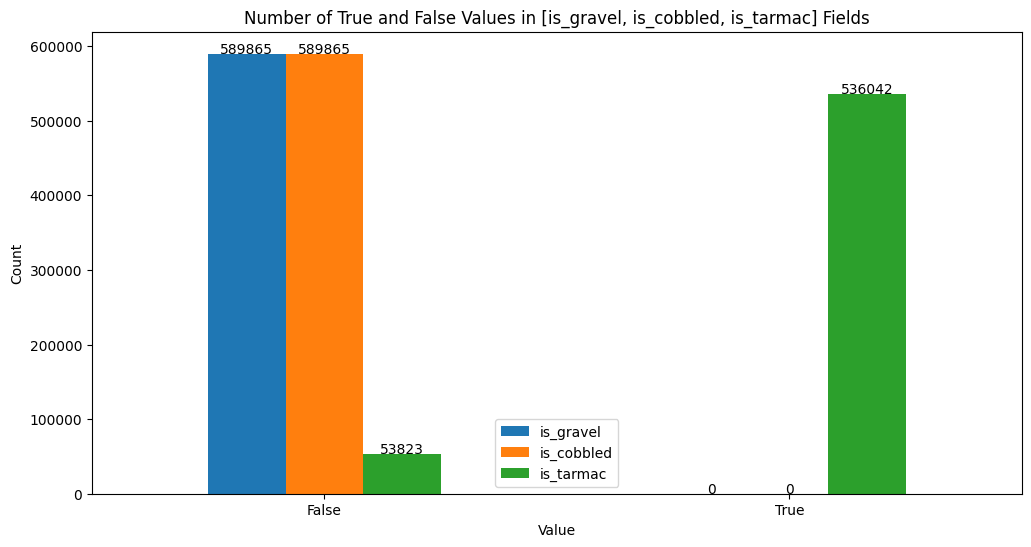
\includegraphics[width=0.55\linewidth]{2.png}
\caption{\label{fig:1}Road type count}
\end{figure}

\begin{figure}
\centering
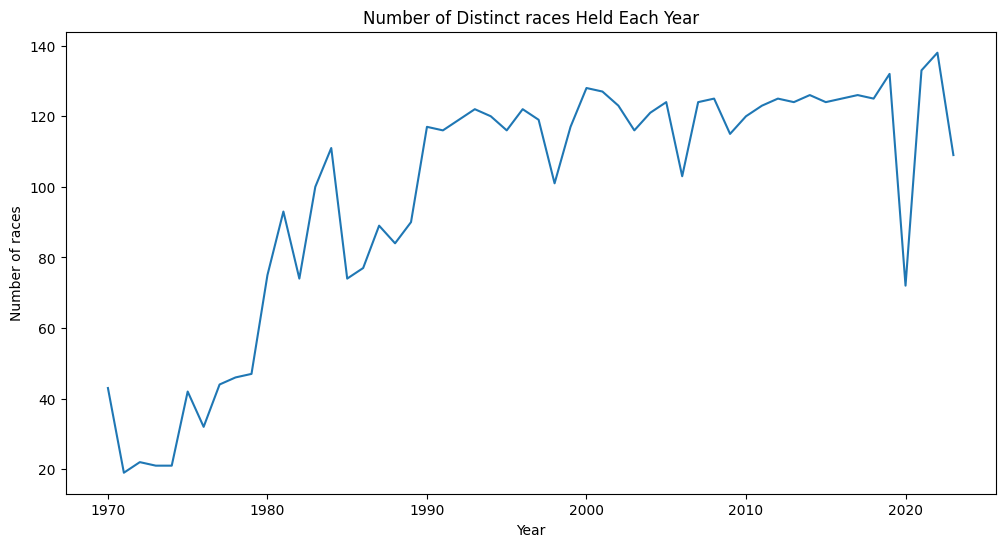
\includegraphics[width=0.55\linewidth]{1.png}
\caption{\label{fig:2}Race number trend over the year}
\end{figure}

\begin{figure}
\centering
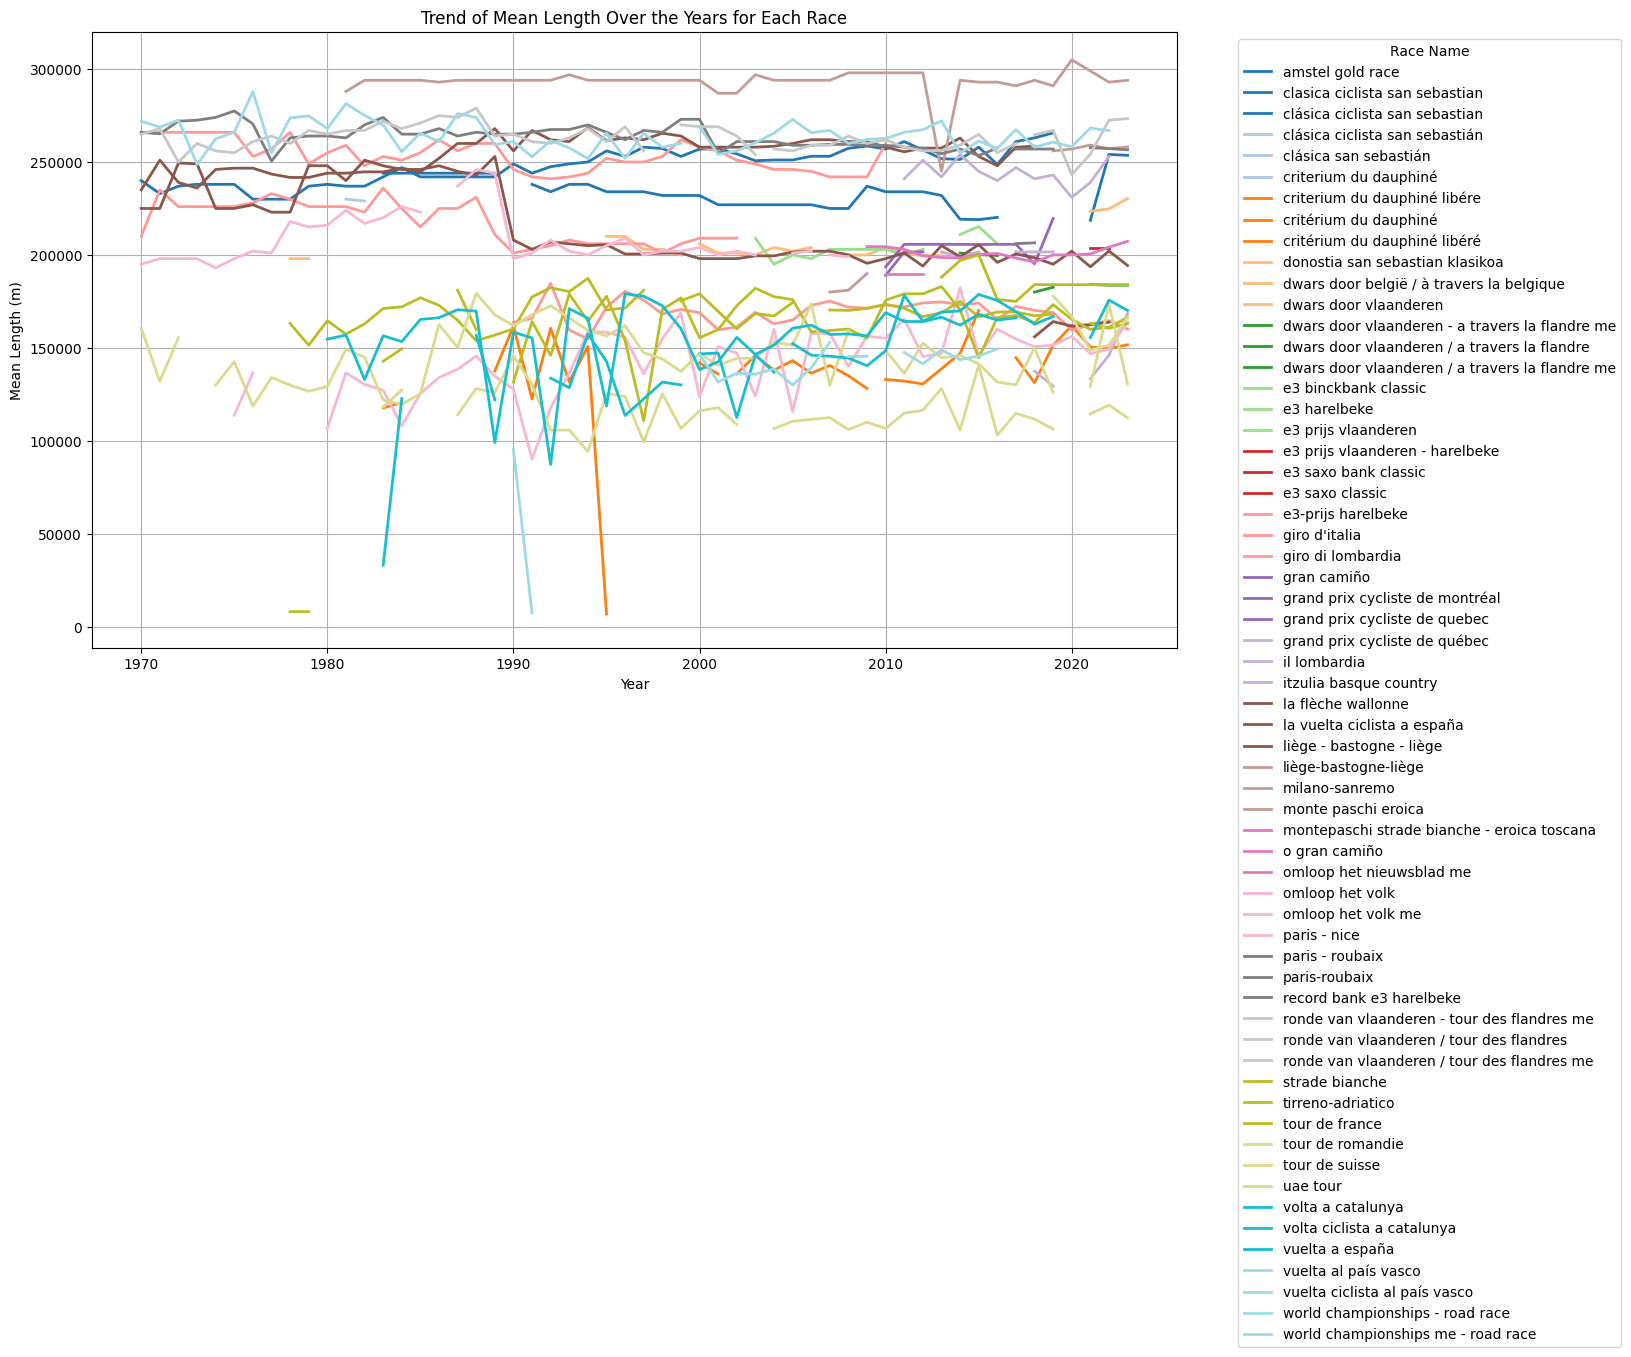
\includegraphics[width=0.40\linewidth]{3.png}
\caption{\label{fig:3}Trend in length of different races over the year}
\end{figure}








\subsection{Handling missing values}

Some attributes have most of the values missing (see fig \ref{missing}), such as 'uci\_points' and 'temperature'. We decided to drop them for they carry no contribution to the analysis.

\begin{figure}[H]
    \centering
    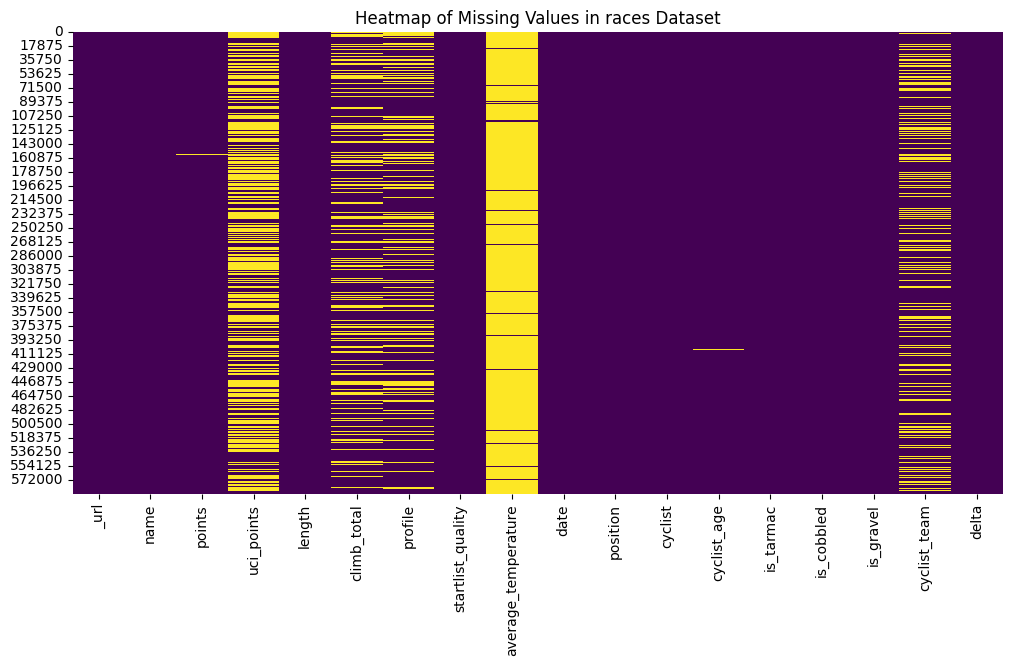
\includegraphics[width=1\linewidth]{missing.png}
    \caption{Missing values in the dataset}
    \label{missing}
\end{figure}


\textbf{Manual fixing}
We found out that in cyclist dataframe, there are 1 missing value in \emph{nationality} and 13 in \emph{birth\_year}. Because the low number, we decided to try to fill them manually by looking for the data in a reliable source and found: 

\begin{enumerate}
    \item \emph{scott davies} with height=184, weight=66, birth year=1995, nationality=great britain 
    
    \url{https://www.wikiwand.com/en/articles/Scott_Davies_(cyclist)
}
    \item  \emph{vladmir malakov} with birth year=1958 
    
    \url{https://www.procyclingstats.com/rider/vladimir-malakov
}
    \item \emph{antonio zanini} with birth year=1965 
    
    \url{https://www.procyclingstats.com/rider/antonio-zanini}
\end{enumerate}


\textbf{Missing birth years}
There are 10 records left with missing [birth\_year] value after manual searching, we decided to fill such records as such:

\begin{enumerate}
    \item look for the first race that cyclist participated in races dataframe
    \item get the mode on the age of cyclists of that year
    \item reverse calculate the [birth\_year] of the cyclist by subtrackting \{year - mode age\}
\end{enumerate}


\textbf{Missing weights and heights}
Weight and height are important and correlated attributes, we decided to fill the missing values by using the following strategy:
To fill the missing values for weight and height while maintaining a normal distribution:

- For missing heights: Fill in with a random value taken from individuals of the same nationality and within a weight range of ±3 kg. If weight is also missing, fill in with a random height taken from individuals of the same nationality.

- For missing weights: Fill in with a random value taken from individuals of the same nationality and within a height range of ±3 cm.

- If there is no value found in the range, we fill with a value from the entire dataset (not only from the same nation).
- For countries with less than 10 individuals, we also use the entire dataset to fill in the missing values.

\textbf{Missing points}
Since there is only a small percentage (477 records = 0.08\%) of missing values on such field, we decided to fill them using the mean of the existing values of the same race stages of the same year.

\textbf{Missing ages}
Since we estimated the cyclists age in the cyclists dataframe, we can now simply calculate the missing values.

\

Data understanding has been repeated after cleaning to verify the correctness of the cleaning process.






\subsection{Data Cleaning and Outlier detection}
\subsubsection{Cyclist - Weight & Height}
Since these attributes follow a normal distribution, we can easily detect (extreme) outliers by using the Inter-quartiles and drop them.
\subsubsection{Races - Points & Races}
The graph \ref{fig:4} shows that the average points for each year before 1977 are unusually high, so we drop races between 1970 and 1977, for they would disrupt the analysis of the dataset. 

The fig \ref{fig:5} shows the average race length of each different race over the year, as already mentioned in the section \emph{before cleaning}, there are 2 sub groups of races. And upon observing, we noticed that longer the race, higher is the points awarded to the cyclist.

\begin{figure}[H]
\centering
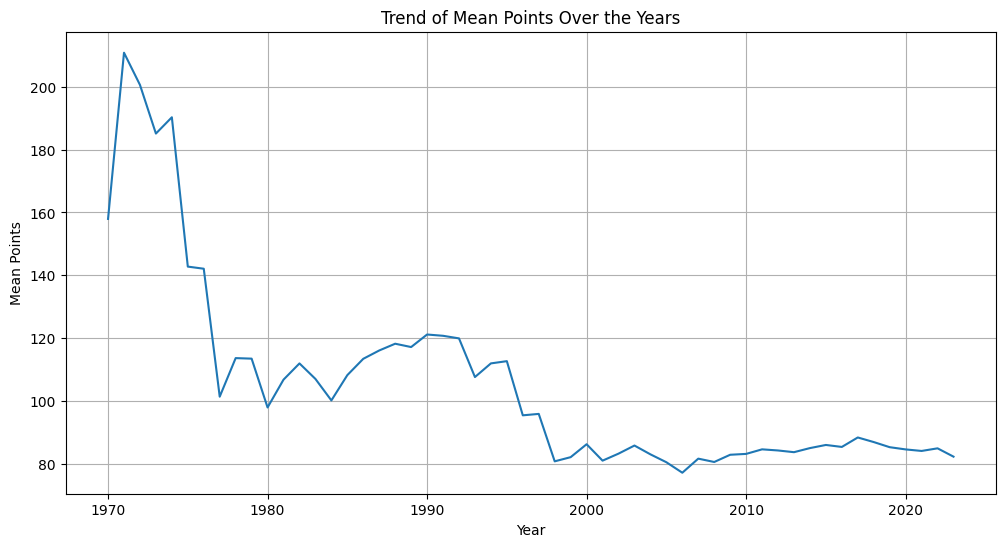
\includegraphics[width=0.40\linewidth]{4.png}
\caption{\label{fig:4}Average awarded points over the year}
\end{figure}

\begin{figure}[H]
\centering
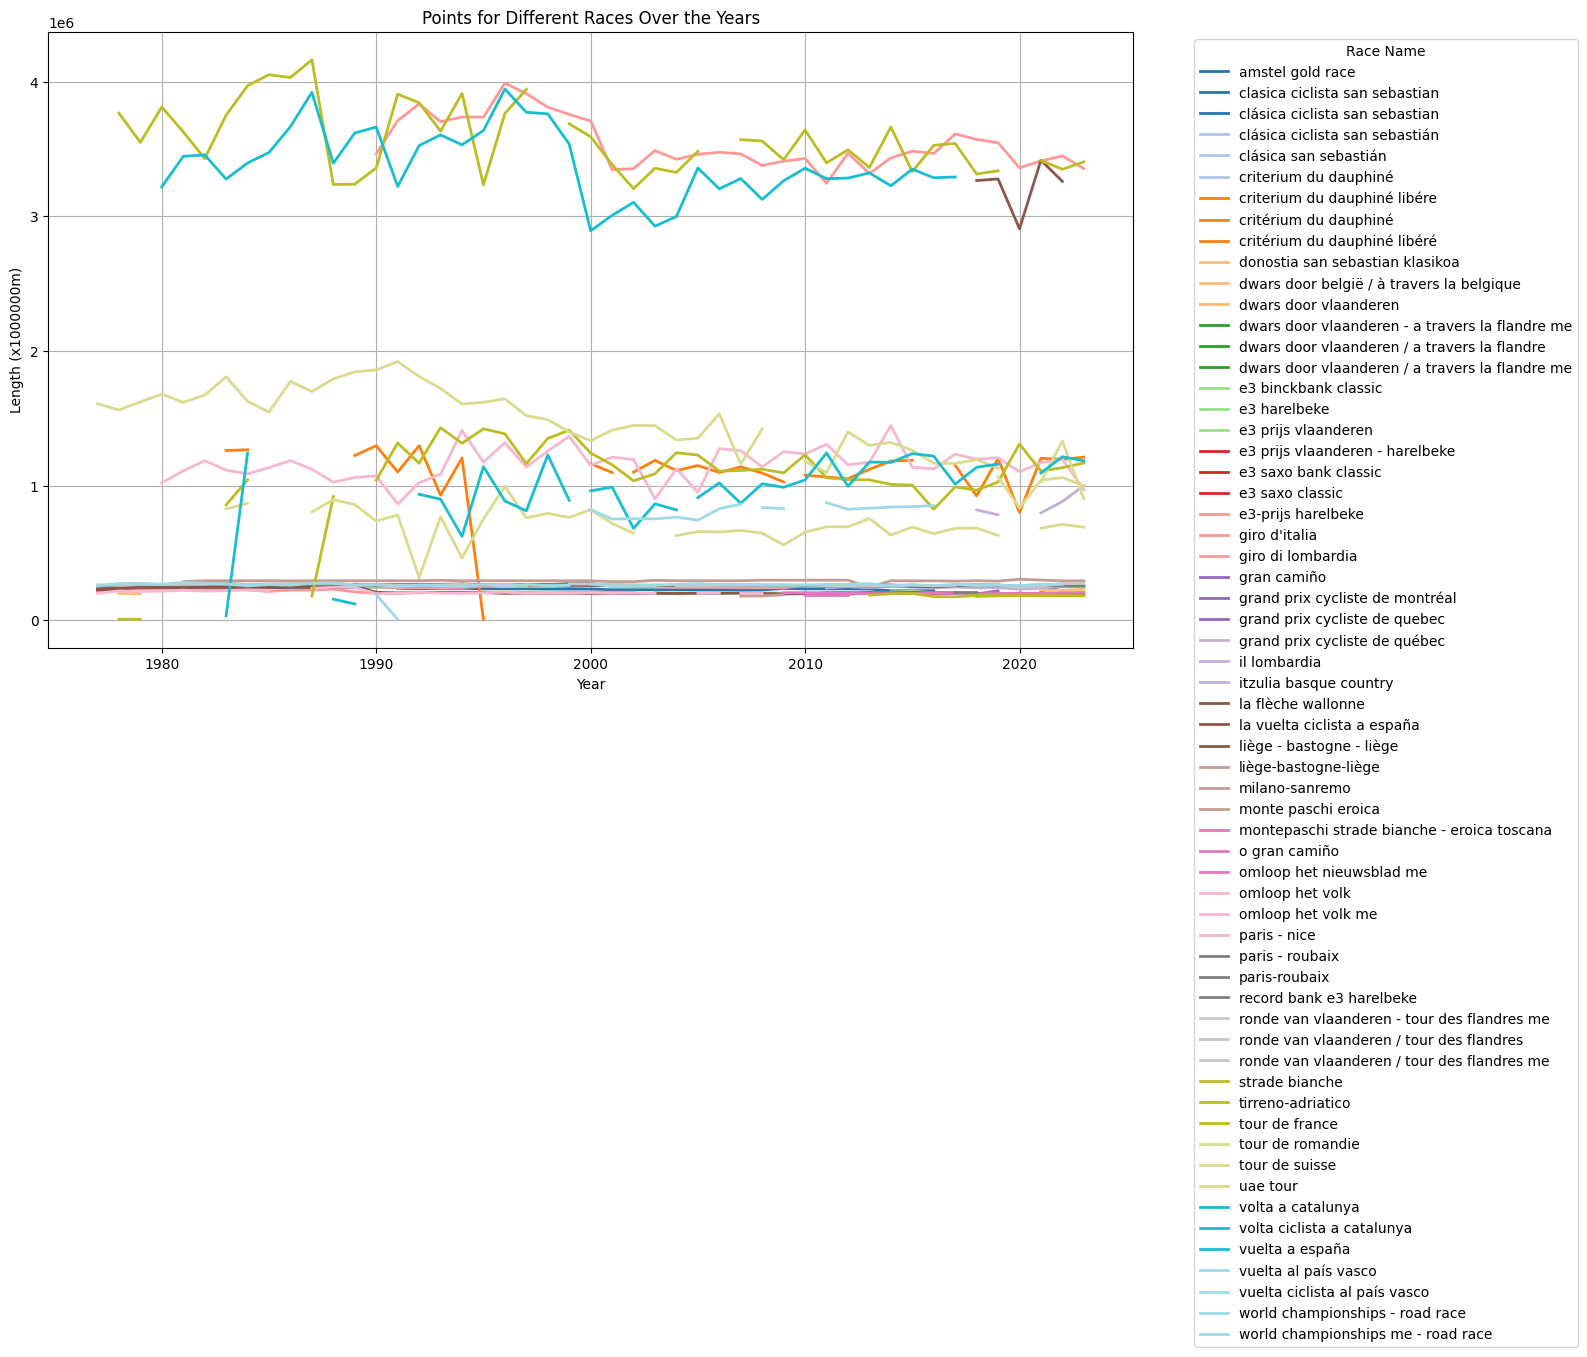
\includegraphics[width=0.40\linewidth]{5.png}
\caption{\label{fig:5}Average individual race length over the year}
\end{figure}

\subsubsection{Races - Cyclist age}
We noticed the presence of a cyclist of age 13 at the time of the race, it is clearly an error and/or outlier, so it has been removed. A cyclist of age over 50 at the time of the race, for it is an extreme value, so it has been removed.

\subsubsection{Cyclists cleaning}
We found out that there are 397 cyclists who are registered in the dataset but have never competed in a single race, they are not interesting to analyze, so we drop them.

Because we updated the cyclist dataframe by removing some of them, we also need to remove the correlated records in races dataframe to maintain consistency.


\subsubsection{New Features}

We added some new features to each cyclist record, in order to better capture the characteristics of the cyclist and of their previous performance.

\begin{enumerate}
    \item BMI - Body Mass Index
    \item races\_participated (total number of races partecipated by the cyclist)
    \item average\_race\_length (average length of races partecipated by the cyclist)
    \item average\_climb\_length (average length of races partecipated by the cyclist on inclined surface)
    \item intensity 
    \item average\_intensity
\end{enumerate}

In figures \ref{fig:distributions} and \ref{fig:boxplots} we show the distribution of the new features and the boxplots of the new features.
We can make some observations:
\begin{itemize}
    \item Many races take place on an entirely flat surface.
    \item Many cyclists only participate to races on a flat surface, as their average\_climb\_total is 0.
    \item The number of races participated by a cyclist is highly skewed, with most cyclists participating in a small number of races, with some outliers participating in more than 300 races.
    \item The average delta follows a quasi-normal distribution, with a considerable number of cyclist arriving at the finish line with a delta of 0 or around 0, meaning they arrived at the same time as the first cyclist.
\end{itemize}

\begin{figure}[H]
\centering
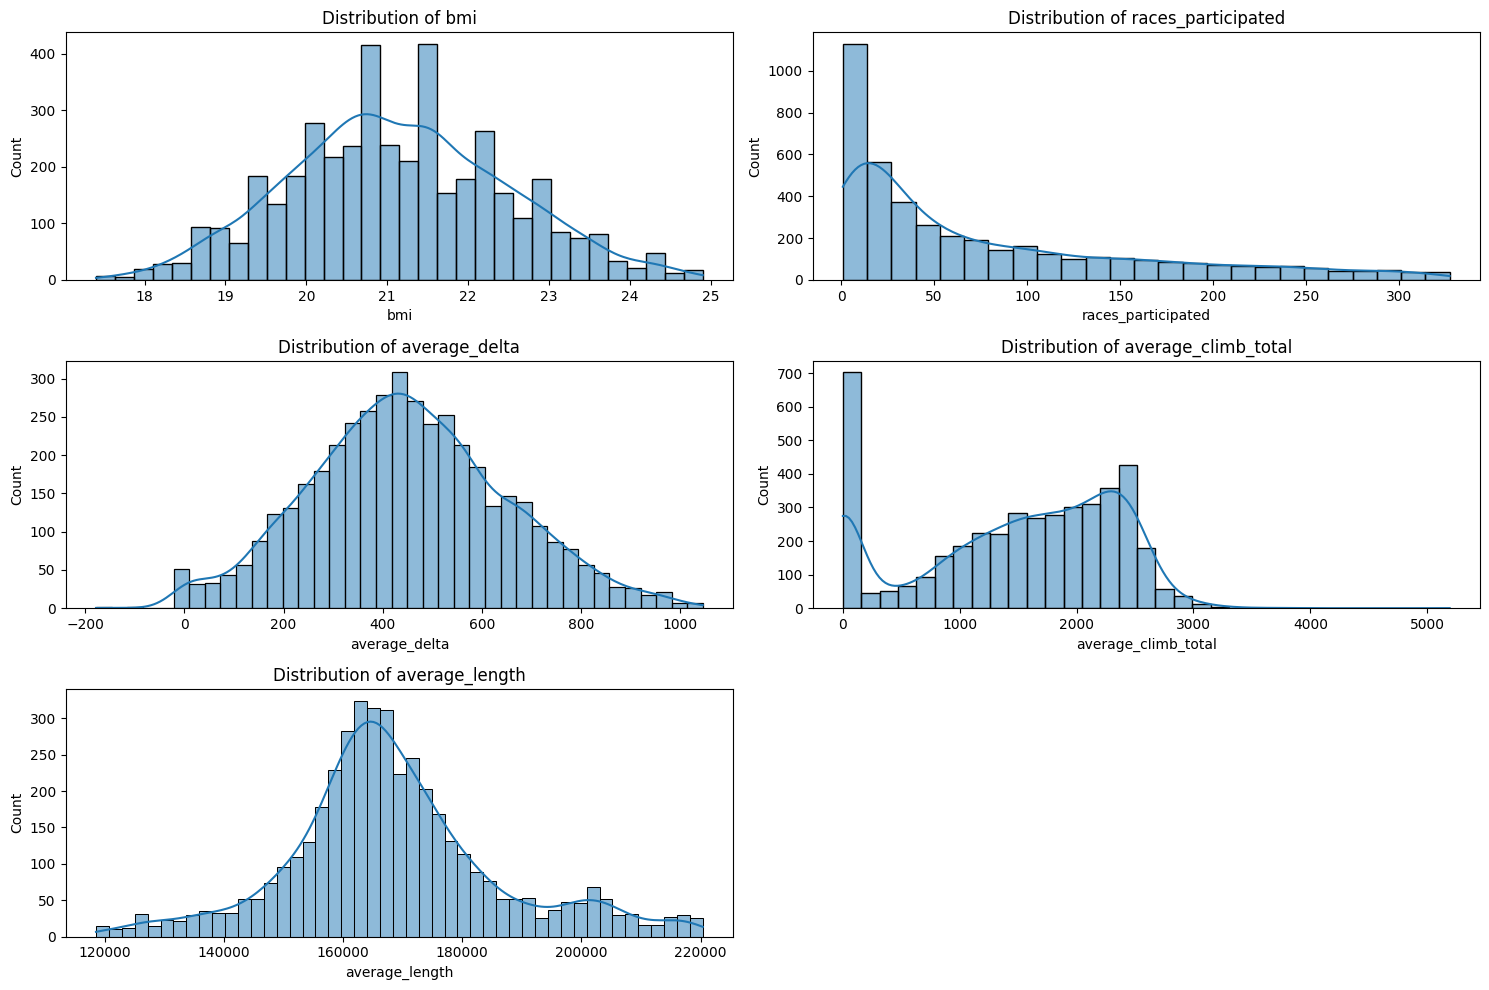
\includegraphics[width=1\linewidth]{distributions.png}
\caption{\label{fig:distributions}Distribution of new features}
\end{figure}

\begin{figure}[H]
\centering
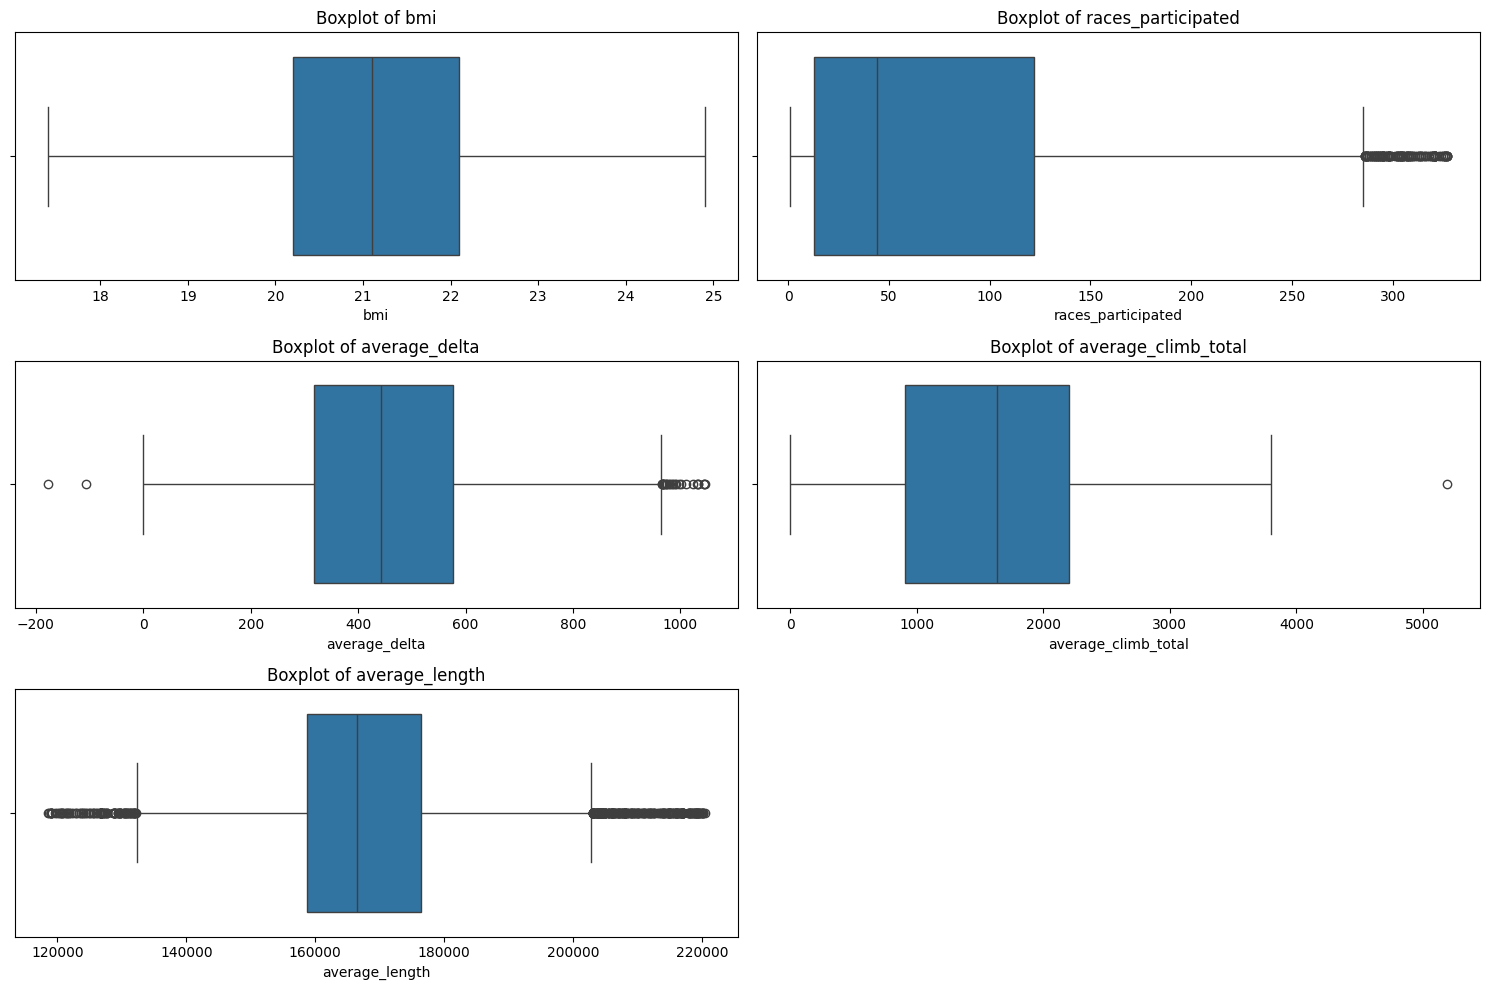
\includegraphics[width=1\linewidth]{boxplots.png}
\caption{\label{fig:boxplots}Boxplots of new features}
\end{figure}
    




\subsection{Attributes and correlation}

\begin{table}[h!]
\centering
\begin{tabular}{|l|l|p{8cm}|l|}
\hline
\textbf{Attribute} & \textbf{Value Type} & \textbf{Description} & \textbf{Data Type} \\ \hline

url\_cyclist & string & Unique identifier of the cyclist & Categorical \\ \hline
name\_cyclist & string & Name of the cyclist formed by name and surname & Categorical \\ \hline
name\_cyclist & string & Name of the cyclist formed by name and surname & Categorical \\ \hline
nationality & string &Nationality of the cyclist & Categorical \\ \hline
birth\_year & int & Birth year of the cyclist & Numerical \\ \hline
weight & int & weight of the cyclist, measured in kg & Numerical \\ \hline
height & int & Height of the cyclist, measured in cm & Numerical \\ \hline
bmi & float & BMI of the cyclist, given by relationship between weight and height & Numerical \\ \hline
races\_participated & int & The number of registered races the cyclists has participated & Numerical \\ \hline
average\_race\_length & int & The average race length the cyclists has run, measured in m & Numerical \\ \hline
average\_climb\_length & int & The average race length on inclined surface the cyclist has run, measured in m & Numerical \\ \hline
average\_intensity & float & The average inclination of the road the cyclist has run on & Numerical \\ \hline

\end{tabular}
\caption{Cyclists dataframe attributes after cleaning}
\label{tab:example}
\end{table}


\begin{table}[h!]
\centering
\begin{tabular}{|l|l|p{8cm}|l|}
\hline
\textbf{Attribute} & \textbf{Value Type} & \textbf{Description} & \textbf{Data Type} \\ \hline

url\_race & string & Unique identifier of the race formed by name/year/stage & Categorical \\ \hline
name\_race & string & Name of the race  & Categorical \\ \hline
points & int & Points awarded to the cyclists & Numerical \\ \hline
length & int & the Total length of the race & Numerical \\\hline
climb\_total & int & The part of the race on inclined surface & Numerical \\\hline
profile & int & Difficulty level of the race & Numerical \\\hline
startlist\_quality & int & How strong a cyclist is & Numerical \\\hline
position & int & The order in which the cyclist arrived at the finish line & Ordinal \\\hline
cyclist & string & The name of the cyclist participating the race & Categorical \\\hline
cyclist\_age & int & The age of the cyclist at the moment of the race & Numerical \\\hline
cyclist\_team & string & The team which the cyclist belongs to & Categorical \\\hline
delta & int & the time difference the cyclist arrives at the finishing line after the first racer & Numerical \\\hline
day & date & The day of the race & Categorical \\\hline
intensity & float & The inclination of the part of inclined road & Numerical \\\hline

\end{tabular}
\caption{Races dataframe attributes after cleaning}
\label{tab:example}
\end{table}

After cleaning, we performed a correlation analysis on the dataset to understand the relationship between the attributes and decide which attributes to use in the analysis - fig \ref{fig:7}.
\begin{figure}[H]
    \centering
    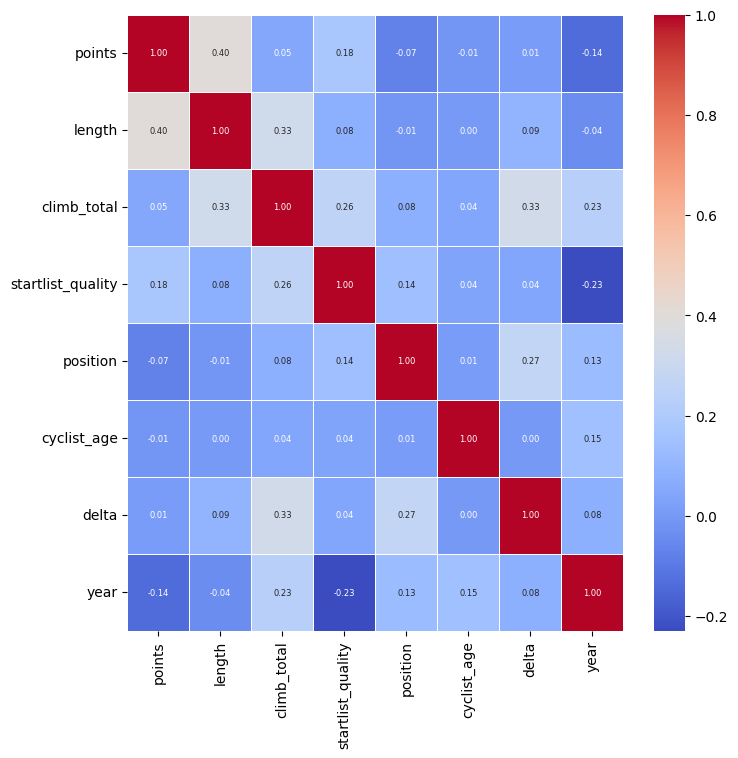
\includegraphics[width=0.50\linewidth]{7.png}
    \caption{\label{fig:7}Correlation matrix on attributes of races}
    \end{figure}



















\section{K-Mean analysis}
The objective is trying to understand how cyclists's physical attributes(weight and bmi) may influence their choice of races (flat, inclined or  both).

We selected features [bmi, weight, average climb length, average race length, average intensity] for they could interprate our goal. We do not want to rank cyclists for there are point-systems already being used officially, we simply want to understand where the physical attribute of a cyclist could influence their choice of race.

We use min-max scaler to normalize the features, because the most of the selected feature have a highly skewed distribution.


For the calculation of the optimal value of clusters k, we used SSE score, Silhouette score and Davies-Bouldin score. Silhourtte measures how well each data point fits within its assigned cluster compared to other clusters. Davies-Bouldin assesses the compactness and separation of clusters in a dataset. Lower values indicate better clustering. After the consideration, we choose k=3. The resulting silhouette score is rounded to 0.3

In fig \ref{fig:8} shows the scatter plot of attributes of clusters

\begin{figure}[H]
\centering
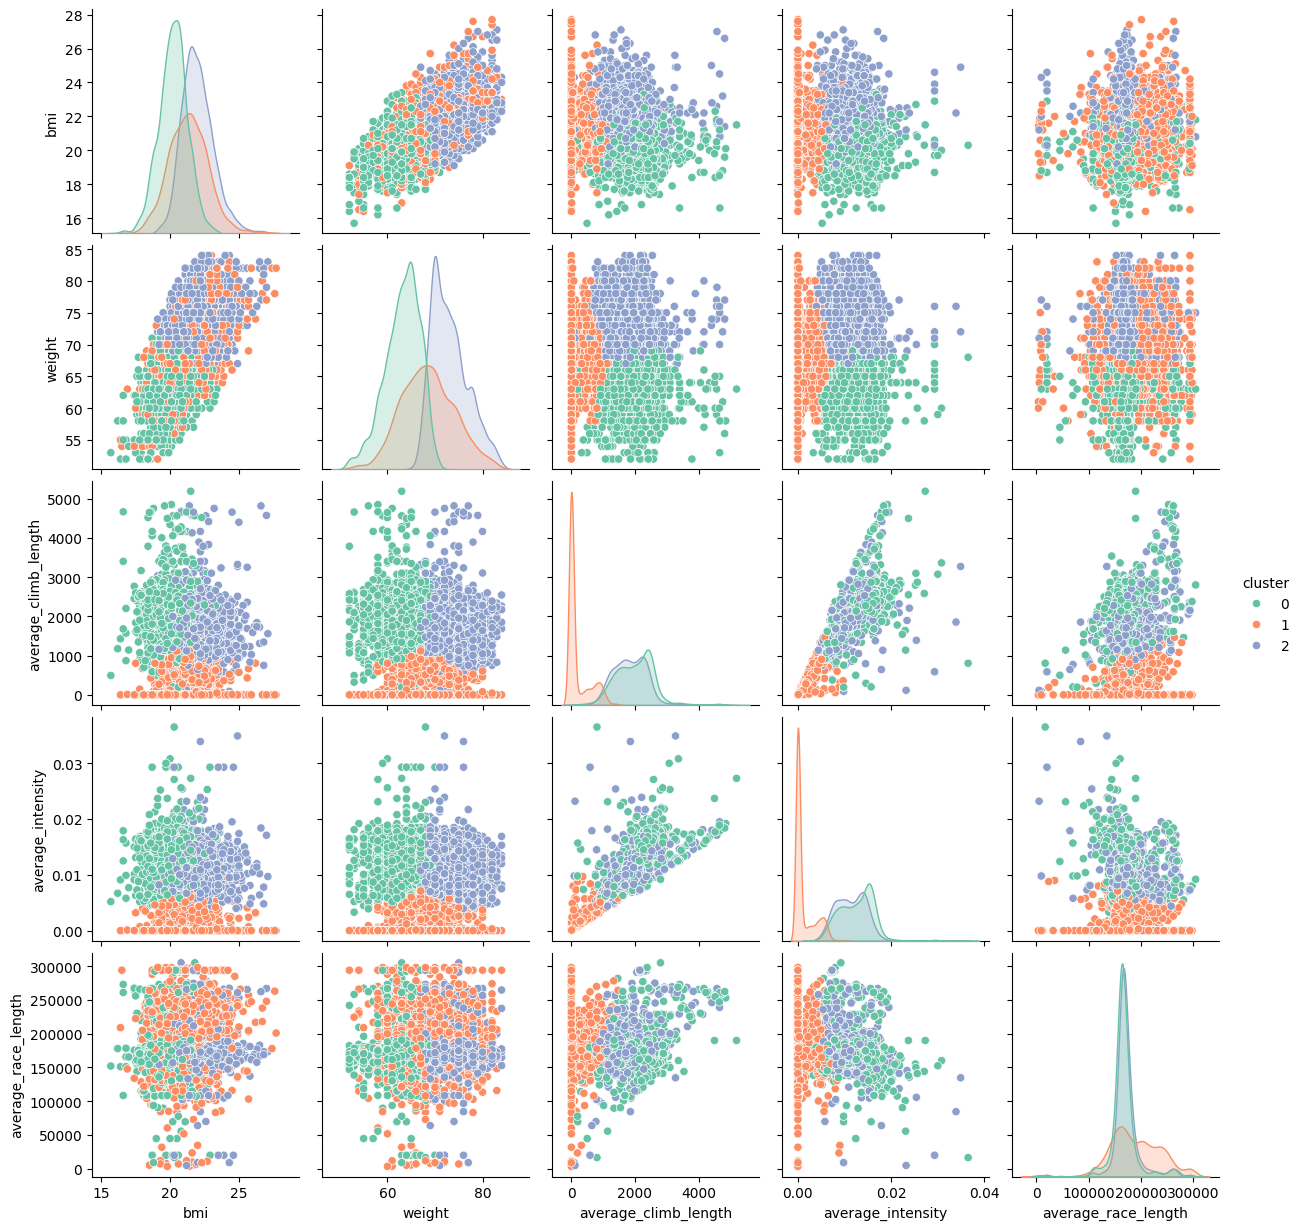
\includegraphics[width=0.40\linewidth]{8.png}
\caption{\label{fig:8}Scatter plot of attributes of clusters}
\end{figure}

In fig \ref{fig:9} shows the importance of each feature used in our analysis, this is calculated through the use of random forest.

\begin{figure}[H]
\centering
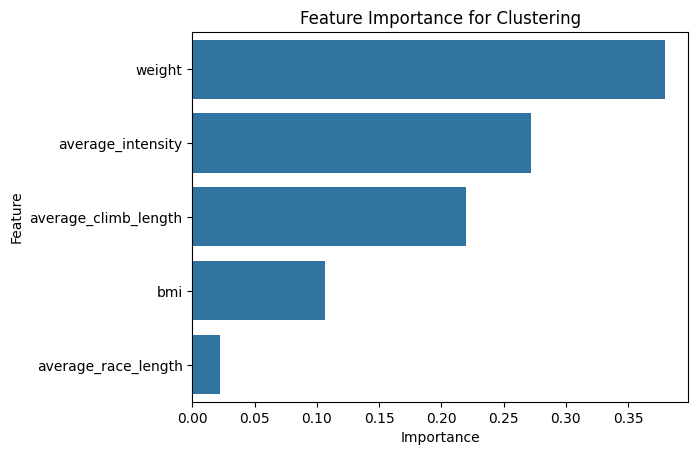
\includegraphics[width=0.40\linewidth]{9.png}
\caption{\label{fig:9}Feature importance in Kmean}
\end{figure}

\subsection{Analysis}
We first ignore the 'average\_race\_length' feature for it is not important in our analysis and also, it shows the similar range of values in all clusters.
In fig \ref{fig:10} shows the centroids of attributes in each cluster:
\begin{enumerate}
    \item cluster 0 has low bmi & weight but high on inclined surface indicators
    \item cluster 1 has high bmi & weight but low on inclined surface indicators.
    \item cluster 2 has high bmi & weight and also high on inclined surface indicators
\end{enumerate}

We observe that: 
\begin{enumerate}
    \item cyclists with lower weight have a higher participation (distance indicators) on inclined surface race. 
    \item cluster 1 are cyclists that don't compete on inclined surface.
    \item cluster 2 are cyclists that can 'feel ease' on both inclined and flat surface
\end{enumerate}

\begin{figure}
\centering
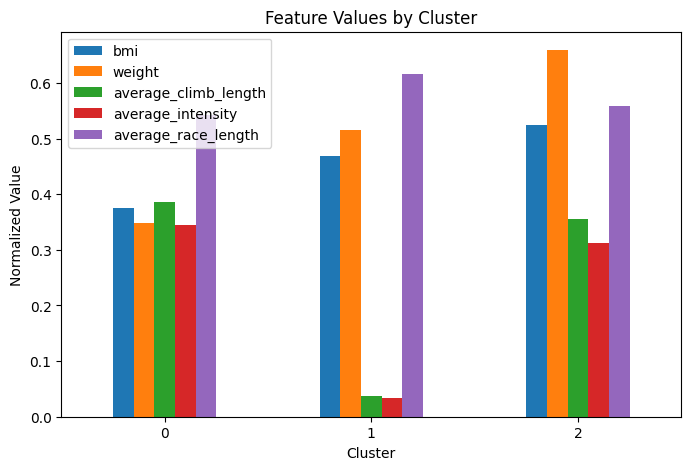
\includegraphics[width=0.55\linewidth]{10.png}
\caption{\label{fig:10}Cluster visualization}
\end{figure}




\section{DBSCAN analysis}
The goal is to understand the preference in the road type (flat or inclined or both) according to their frequency in competing. 

We select features ['races participated', 'average race length', 'average climb length', 'average intensity'] and again, use min-max scaler to normalize them. 

The method requires 2 hyperparameter, eps and min sample. The eps is the maximum radius of the neighborhood around a point to be considered part of the same cluster. And we try to find the value by using both KNN method and Knee method where in KNN, the 'imaginary' min sample is 2*number of features while in Knee, the distance between pairwise points are calculated using euclidean. We find out that the best eps ranges in [0.04, 0.08], so we attempted to find the best combination of eps and min sample by varing eps in its range and varing min sample in [2, 9], and use silhouette score as metrics. 

In fig \ref{fig:11} shows the silhouette score of the combination, according to the results, combinations with eps={0.06, 0.07, 0.08} and min sample={7, 8} produce almost equivalently good results, so we decided to choose arbitrary epq=0.07 and min sample=7. And also, these combinations don't produce a large nor too little number of clusters.

\begin{figure}
\centering
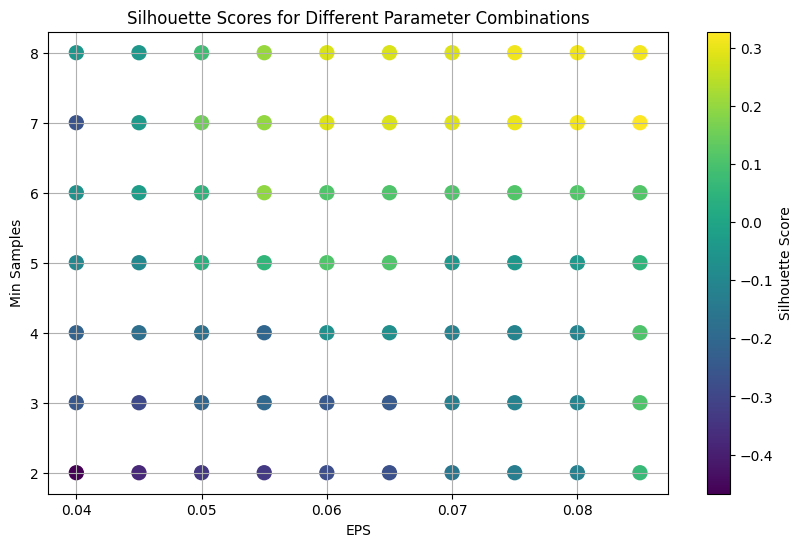
\includegraphics[width=0.40\linewidth]{11.png}
\caption{\label{fig:11}Silhouette score of eps/min sample combinations}
\end{figure}

\subsection{Analysis}
With the parameters, we proceeded with DBSCAN on the datasets and produced 4 clusters. 
\begin{enumerate}
    \item cluster 1 functions as the baseline for the dataset, where majority of cyclists belong to,they have consistant preference in road type
    \item cluster 0 has 12 members, acting like a singularity, after analyzing the results, we discover that this cluster has only cyclists that have run 1 specific race they are low in the races length, both on flat and inclined surface. But the race they run on has a high(er) percentage of inclined surface, this could impliy that they were a subset of specialized cyclists for the race.
    \item cluster 3 has 14 members, with low results on all features, we can deduce that the cyclists in this cluster are less experienced racers.
    \item cluster 2 has 36 members, even with low participation, they achieve high results on other feature, we can categorize them as above average cyclists experienced on different type of races.
    \item cluster -1 (outliers)  with 77 members, are a mix of extremely experienced cyclists with high number of race participation but below average performance, underperforming cyclists, elits cyclists and data-anomalies.
\end{enumerate}






\section{Hierarchical Analysis}

\subsection{Objective}
The goal of this analysis is to understand the types of cyclists based on their race metrics (average climb length, average race length), experience (number of races participated), and physical attributes (weight). We aim to categorize cyclists into clusters that reflect their characteristics and preferences in race types.

\subsection{Data Preprocessing}
To minimize noise, we filtered the dataset by removing extreme values, keeping only records within the 5th to 95th percentiles of the \texttt{races\_participated} feature.


The selected features for clustering are:
\begin{itemize}
    \item \texttt{weight}
    \item \texttt{races\_participated}
    \item \texttt{average\_race\_length}
    \item \texttt{average\_climb\_length}
    \item \texttt{average\_intensity}
\end{itemize}

We used MinMaxScaler to normalize these features due to their highly skewed distributions.

\subsection{Clustering Methodology}
Using hierarchical clustering, we calculated the Euclidean distance between data points and employed the complete linkage method. The dendrogram in Figure \ref{fig:dendrogram} illustrates the hierarchical clustering structure.

\begin{figure}[H]
    \centering
    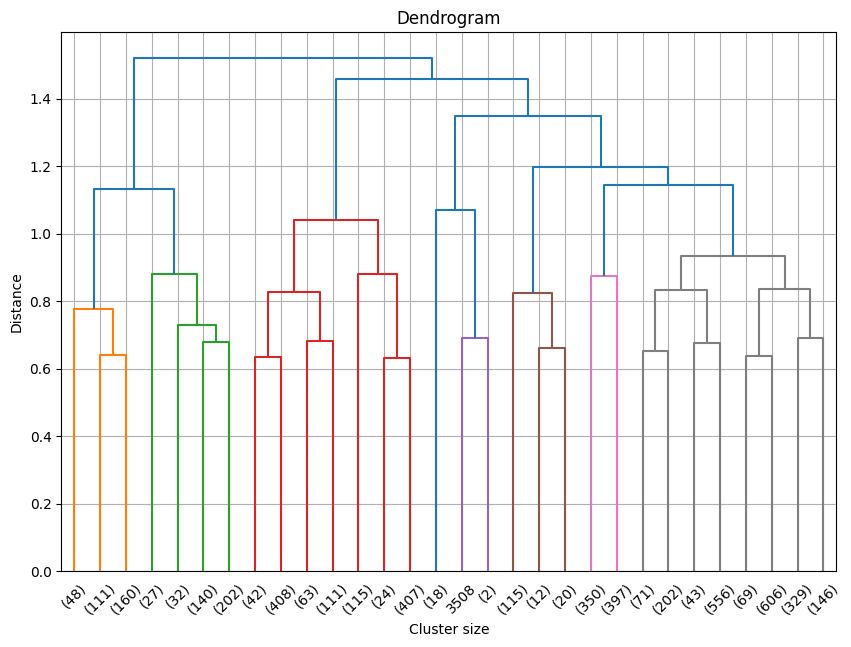
\includegraphics[width=0.4\linewidth]{dend.png}
    \caption{Dendrogram of Hierarchical Clustering}
    \label{fig:dendrogram}
\end{figure}

We chose to cut the dendrogram at a distance of 1.2, resulting in four clusters.

\subsection{Cluster Analysis}

The characteristics of each cluster are summarized below, based on the mean values of the selected features within each cluster.

\begin{itemize}
    \item \textbf{Cluster 0}: Cyclists with moderate \texttt{weight}, \texttt{races\_participated}, and \texttt{average\_climb\_length}. They represent average cyclists experienced in both flat and inclined races but not as seasoned as Cluster 2.
    \item \textbf{Cluster 1}: Cyclists with the lowest \texttt{weight} and highest \texttt{average\_climb\_length}. They are skilled in inclined surface races.
    \item \textbf{Cluster 2}: Cyclists with the highest \texttt{races\_participated} and high values for other metrics. These are experienced cyclists proficient in both flat and inclined races.
    \item \textbf{Cluster 3}: Cyclists with the lowest values across all metrics, indicating they are less experienced racers.
\end{itemize}

\begin{figure}[H]
    \centering
    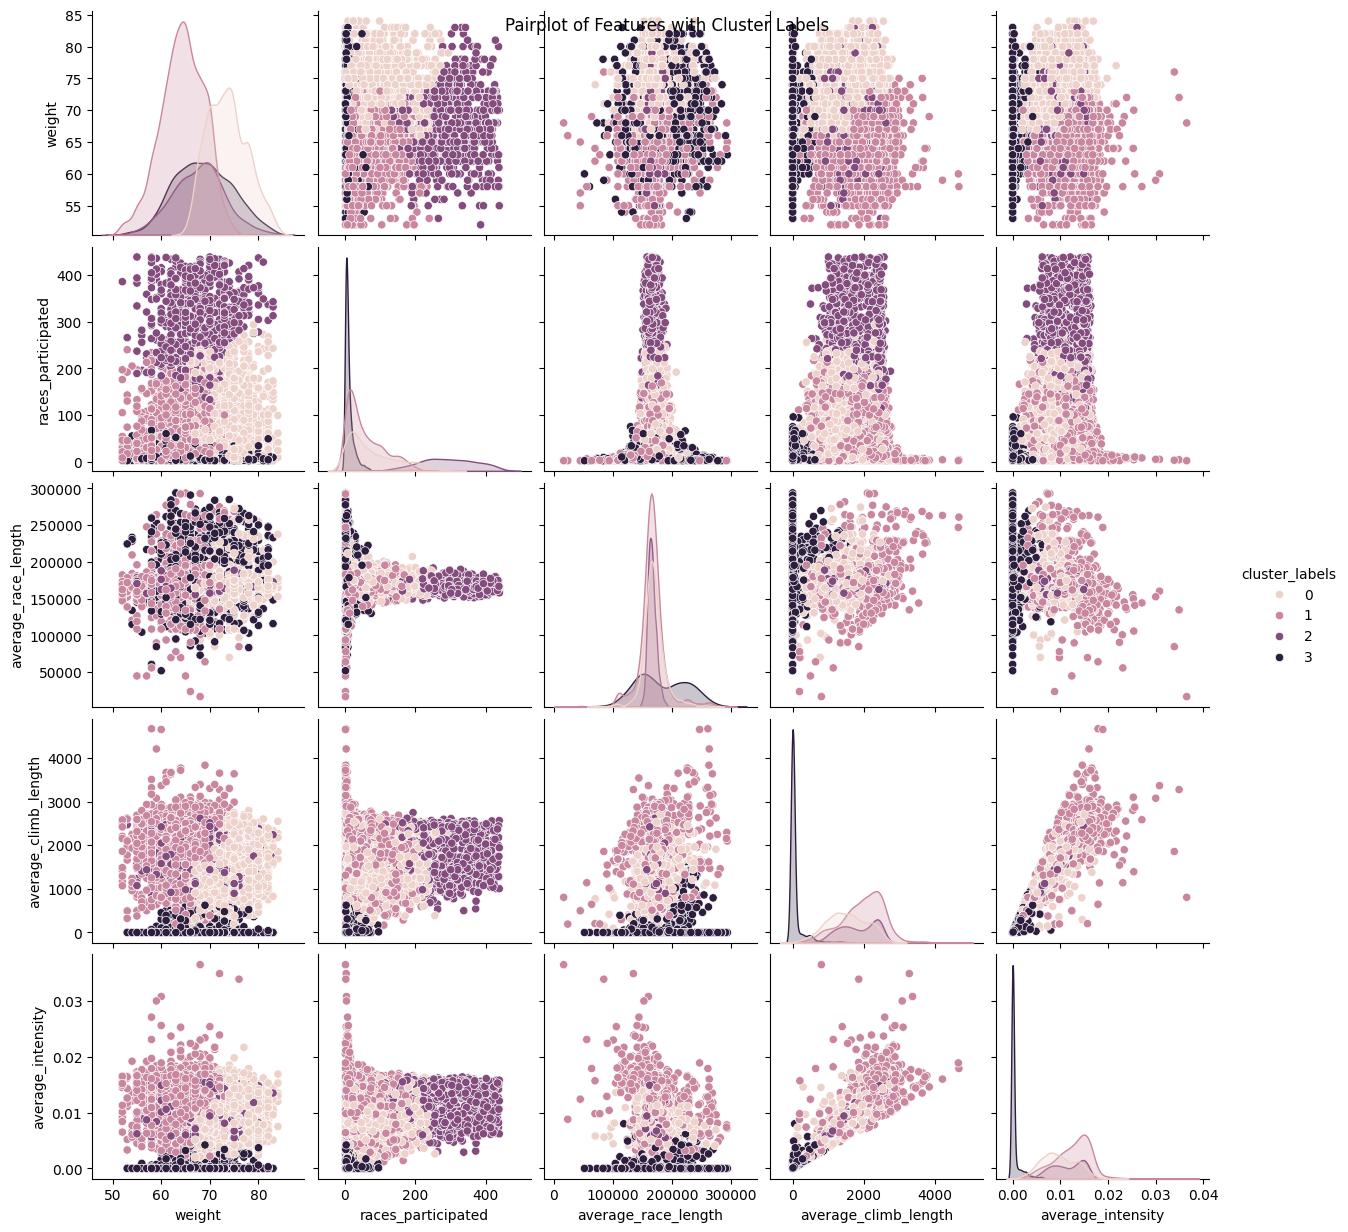
\includegraphics[width=0.8\linewidth]{dend_pair.png}
    \caption{Cluster Visualization by Feature}
    \label{fig:cluster_visualization}
\end{figure}

\subsection{Feature Importance}
Using a Random Forest classifier, we evaluated the importance of each feature in distinguishing between clusters. The results, shown in Figure \ref{fig:feature_importance}, indicate that \texttt{races\_participated} and \texttt{weight} are the most critical features.

\begin{figure}[H]
    \centering
    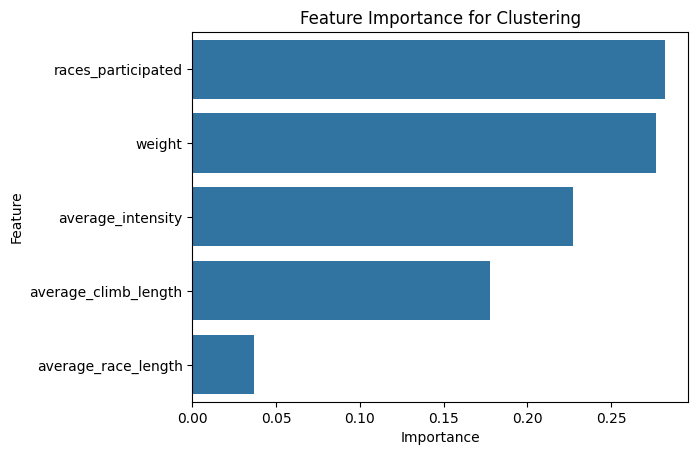
\includegraphics[width=0.55\linewidth]{feature_importance_dend.png}
    \caption{Feature Importance for Hierarchical Clustering}
    \label{fig:feature_importance}
\end{figure}

\subsection{Observations}
\begin{itemize}
    \item \textbf{Cluster 3} includes cyclists with minimal race participation and low physical metrics, suggesting they are less experienced.
    \item \textbf{Cluster 2} features the most experienced cyclists, excelling in various race types.
    \item \textbf{Cluster 1} highlights cyclists specializing in races with significant climbs.
    \item \textbf{Cluster 0} represents average cyclists proficient in multiple race types but less seasoned than those in Cluster 2.
\end{itemize}

The silhouette score for this clustering is 0.26, indicating moderate clustering performance.

\subsection{Conclusion}
The hierarchical clustering analysis effectively categorized cyclists based on physical attributes and race metrics, revealing insights into their preferences and specialization in race types.















\section{Prediction task}

We evaluated five different types of prediction models to determine the most effective approach for our dataset. The dataset was divided into training, validation, and test sets. As per the project requirements, the test set included races from 2022 onward. This test set was used only once, after the models were selected, to ensure unbiased performance evaluation.

\subsection{Data Preprocessing}
\subsubsection{Label Calculation}
For each record in the dataset, we calculated the \texttt{is\_top\_20} label, indicating whether a cyclist ranked in the top 20. We observed that only 14.8\% of the records had \texttt{is\_top\_20=true} \ref{fig:beforeunders}, creating a significant class imbalance. To address this, we undersampled the majority class to achieve a balanced 50\%/50\% class distribution \ref{fig:afterunders}.

We observed that the itorduction of the undersampling technique significantly improved the recall for the minority class (\texttt{is\_top\_20=true}), which would otherwise have been underrepresented.

\begin{figure}[H]
    \centering
    \begin{minipage}{0.45\linewidth}
        \centering
        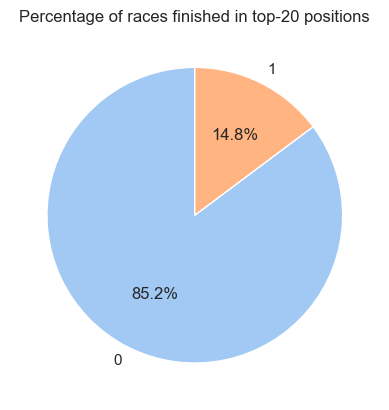
\includegraphics[width=\linewidth]{beforeunders.png}
        \caption{Before undersampling}
        \label{fig:beforeunders}
    \end{minipage}
    \hfill
    \begin{minipage}{0.45\linewidth}
        \centering
        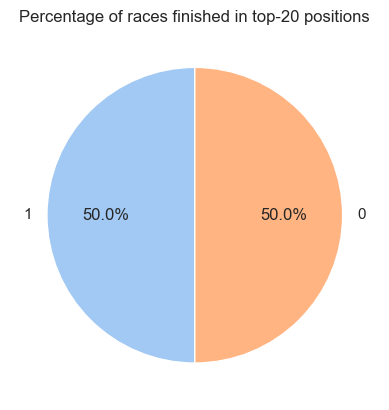
\includegraphics[width=\linewidth]{afterunders.png}
        \caption{After undersampling}
        \label{fig:afterunders}
    \end{minipage}
\end{figure}

\subsubsection{Discretization and Feature Selection}
We applied one-hot encoding to discretize the categorical data, which improved the model's performance compared to numerical discretization methods. Additionally, we selected the relevant features for prediction and excluded those that were either irrelevant or features that should be unavailable until the race finishes. This feature selection process ensured that the models focused only on the most useful information.

\subsection{Model Evaluation}
Each model was evaluated using precision, recall, F1-score, and support metrics on both the training and validation sets. We used visualizations such as confusion matrices and ROC curves for a clearer understanding of each model's performance.

\subsubsection{K-Nearest Neighbors (KNN)}
We performed a grid search to optimize the parameters for \texttt{k}, the distance metric, and the weight strategy. The best parameters found were:
\begin{verbatim}
{'weights': 'distance', 'n_neighbors': 20, 'metric': 'manhattan'}
\end{verbatim}

Performance on the validation set was as follows:
\begin{verbatim}
              precision    recall  f1-score   support

  Not Top-20       0.77      0.72      0.74      9172
      Top-20       0.73      0.78      0.76      9195

    accuracy                           0.75     18367
   macro avg       0.75      0.75      0.75     18367
weighted avg       0.75      0.75      0.75     18367
\end{verbatim}

We observe that the KNN model performed well, with balanced precision and recall.

\subsubsection{Naive Bayes}
Naive Bayes was tested on the training set, and its performance is summarized below:
\begin{verbatim}
Report of the performance on the VALIDATION set:
              precision    recall  f1-score   support

  Not Top-20       0.62      0.65      0.64      9172
      Top-20       0.63      0.61      0.62      9195

    accuracy                           0.63     18367
   macro avg       0.63      0.63      0.63     18367
weighted avg       0.63      0.63      0.63     18367
\end{verbatim}

\textbf{Observation:} The Naive Bayes model struggled with classifying the set correctly, maybe due to its strong assumptions of feature independence.

\begin{figure}[H]
    \centering
    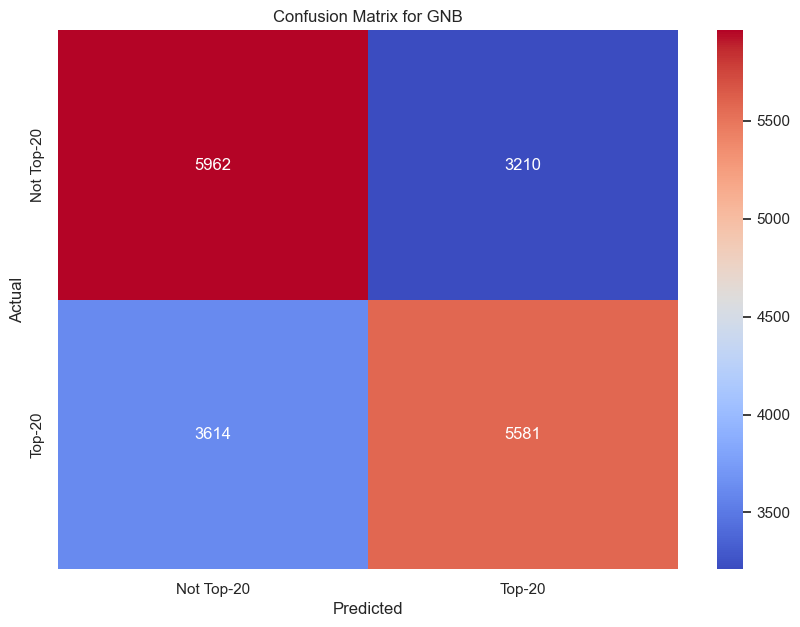
\includegraphics[width=0.5\linewidth]{gnb.png}
    \caption{Confusion matrix for Naive Bayes}
    \label{fig:enter-label}
\end{figure}


\subsubsection{Rule-Based (RIPPER)}
Given the high computational cost, we opted for \texttt{RandomizedSearchCV} for parameter tuning. The best parameters identified were:
\begin{verbatim}
{'prune_size': 0.3, 'k': 1}
\end{verbatim}

Performance on the training set:
\begin{verbatim}
Report of the performance on the VALIDATION set:
              precision    recall  f1-score   support

  Not Top-20       0.55      0.97      0.70      9172
      Top-20       0.87      0.23      0.36      9195
\end{verbatim}

\textbf{Observation:} While the RIPPER algorithm achieved high precision for the minority class, its recall was very low.


\begin{figure}[H]
    \centering
    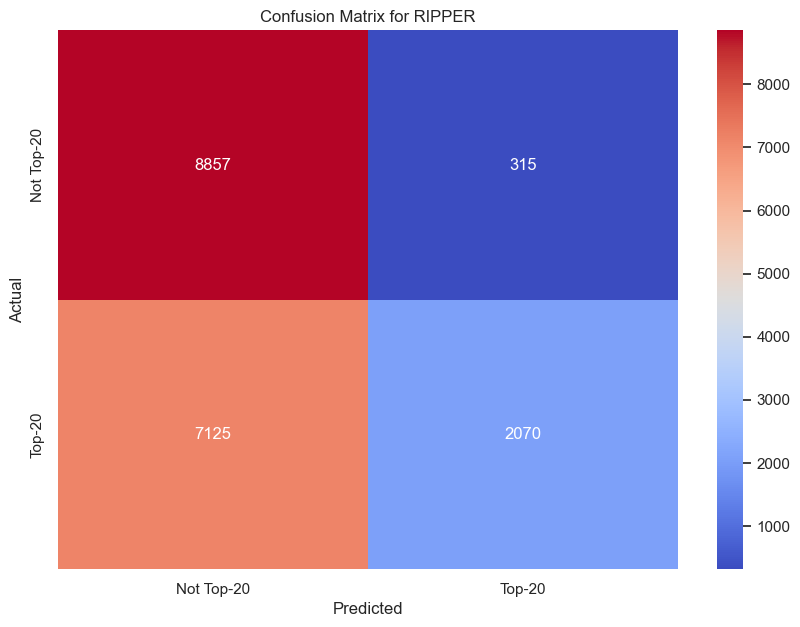
\includegraphics[width=0.5\linewidth]{confusion_ripper.png}
    \caption{Confusion matrix for RIPPER}
    \label{fig:enter-label}
\end{figure}




\subsubsection{Decision Trees}
We conducted a grid search over many parameter combinations.
The training process was fast, and the best parameters found were:
\begin{verbatim}
{'criterion': 'entropy', 'max_depth': 7, 'min_samples_leaf': 4, 'min_samples_split': 2, 'splitter': 'best'}
\end{verbatim}

Performance:
\begin{verbatim}
Report of the performance on the VALIDATION set:
              precision    recall  f1-score   support

  Not Top-20       0.67      0.73      0.70      9172
      Top-20       0.70      0.64      0.67      9195

    accuracy                           0.68     18367
   macro avg       0.68      0.68      0.68     18367
weighted avg       0.68      0.68      0.68     18367
\end{verbatim}

\textbf{Observation:} Decision Trees showed a good balance between precision and recall, but its performance was not as high as KNN. there might be potential room for improvement in parameter tuning.

\subsubsection{Neural Network (Keras)}
The Keras-based neural network model was structured as follows:
\begin{verbatim}
keras_model = tf.keras.Sequential([
    Input(shape=(train_set_scaled.shape[1],)),
    Dense(128, activation='relu', kernel_regularizer=l2(0.001)),
    Dropout(0.3),
    Dense(64, activation='relu', kernel_regularizer=l2(0.001)),
    Dropout(0.3),
    Dense(32, activation='relu', kernel_regularizer=l2(0.001)),
    Dropout(0.3),
    Dense(1, activation='sigmoid')
])
keras_model.compile(
    optimizer='adam',
    loss='binary_crossentropy',
    metrics=[tf.keras.metrics.BinaryAccuracy(), tf.keras.metrics.Precision(), tf.keras.metrics.Recall(), tf.keras.metrics.AUC()]
)
\end{verbatim}

We selected this architecture because it is well-suited for binary classification tasks. We experimented with various architectures and parameters, and this one gave the best results. Although we chose the 'binary-cross-entropy' loss function, our evaluation considered multiple factors \ref{fig:kerasmetrics}. We manually tuned some parameters for optimal performance.

\begin{figure}[H]
    \centering
    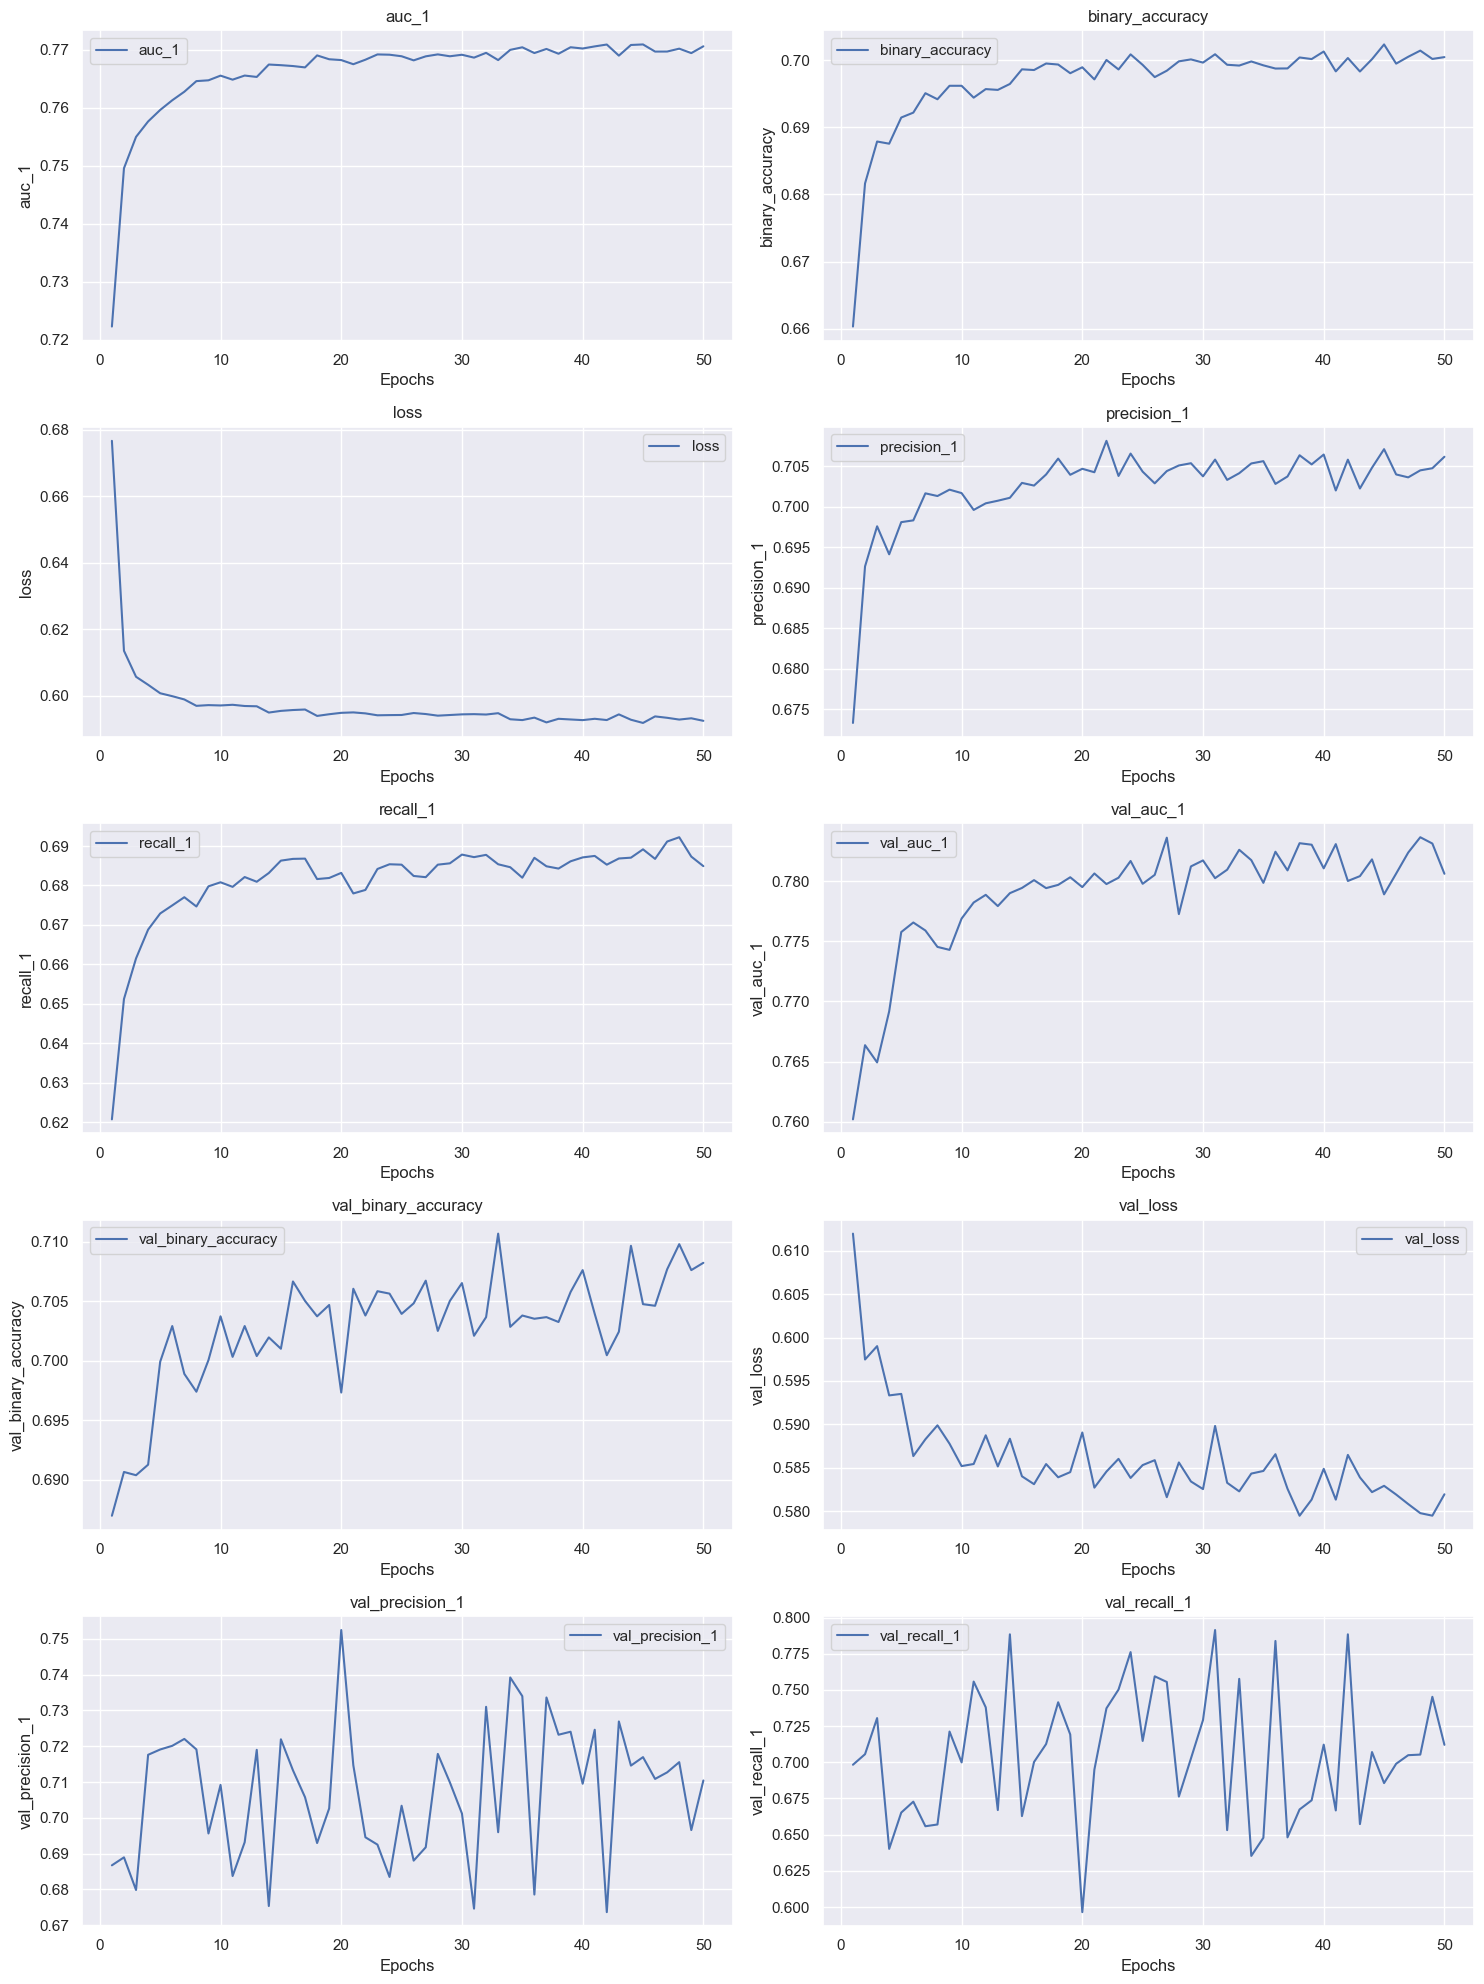
\includegraphics[width=1.0\linewidth]{kerasmetrics.png}
    \caption{Some of the metrics taken into consideration while tuning the Keras model}
    \label{fig:kerasmetrics}
\end{figure}



Performance on the training set:
\begin{verbatim}
              precision    recall  f1-score   support

  Not Top-20       0.72      0.72      0.72      9172
      Top-20       0.72      0.73      0.72      9195
\end{verbatim}
It shows a good precision and recall, balanced for both classes.
























\subsection{Model Comparison}
We compared the models using ROC curves to visualize their performance:
\begin{itemize}
    \item KNN (AUC = 0.75)
    \item GNB (AUC = 0.63)
    \item RIPPER (AUC = 0.60)
    \item Decision Tree (AUC = 0.68)
    \item Keras (AUC = 0.72)
\end{itemize}

\begin{figure}[H]
    \centering
    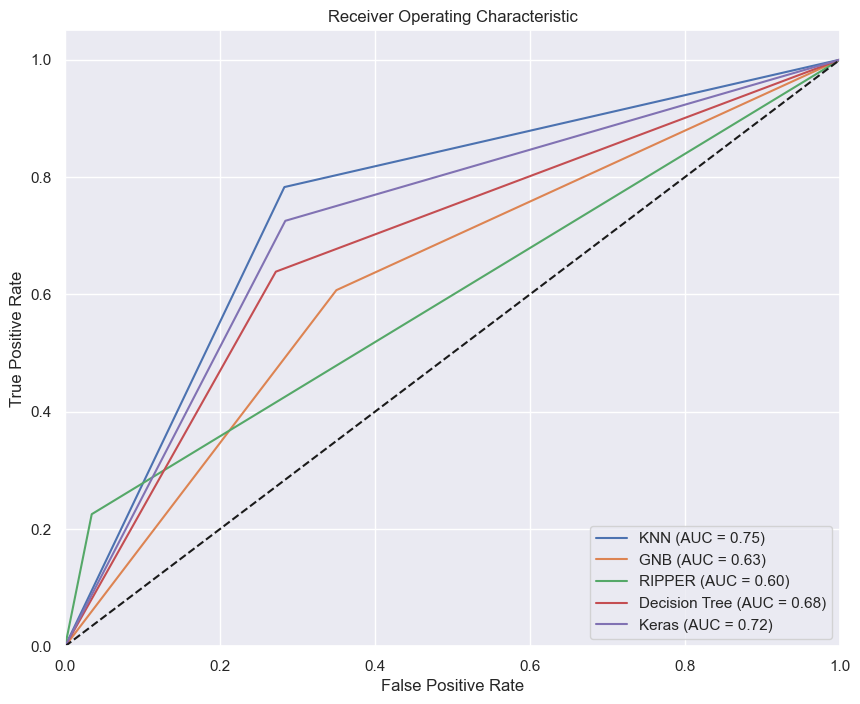
\includegraphics[width=0.8\linewidth]{valset.png}
    \caption{ROC for the validation set}
    \label{fig:enter-label}
\end{figure}

The KNN model had the highest AUC, followed by the neural network. RIPPER, with the lowest AUC, struggled to handle the complexity of the dataset.

\section{Test Set Results}
To conclude, we evaluate the best 3 models on the test set. 
To avoid introducing bias, the test set has been used only once.

The performance of the Decision Tree model dropped significantly in the test set, highlighting potential overfitting during training.

KNN and the neural network generalized better than the decision tree, though the recall on the minority class dropped.


\begin{figure}[H]
    \centering
    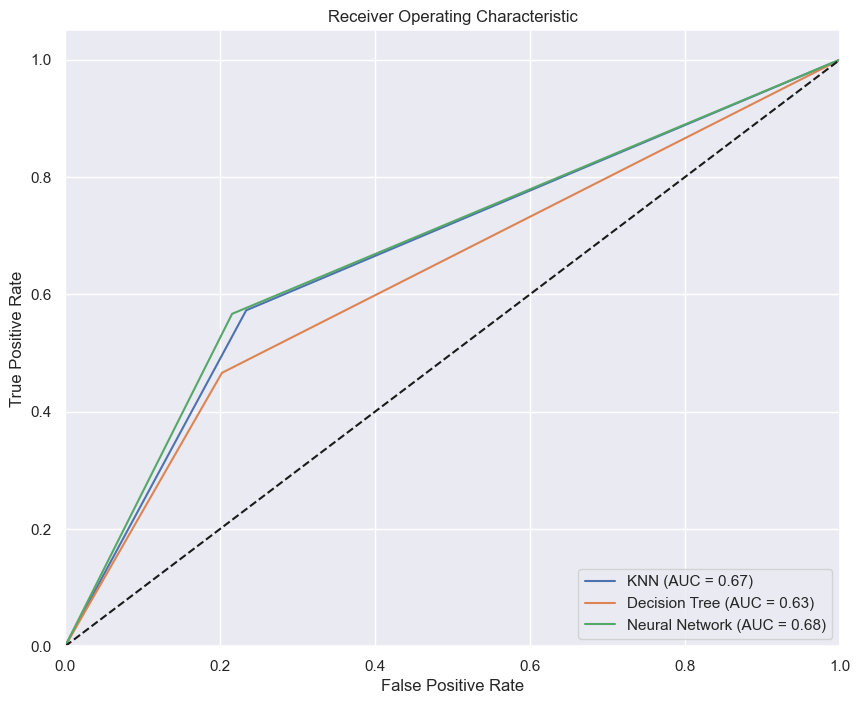
\includegraphics[width=0.5\linewidth]{testset.png}
    \caption{ROC on the test set}
    \label{fig:enter-label}
\end{figure}

































\section{Explanation}

\subsection{Introduction}
In this section, we provide explanations for some of the machine learning models we developed and selected in the previous task We will explore aspects such as feature importance, rule explanations, and counterfactual instances.

\subsection{Overview of Selected Models}
We chose to focus on two distinct models: the Decision Tree (DT) and the Keras Neural Network (NN). These models were selected because they performed well in the previous task and offer an interesting contrast in terms of complexity and interpretability. The Decision Tree is straightforward and easy to interpret, while the Neural Network is more complex and harder to interpret.


\subsection{Explaination for the Decision Tree Model}


\subsubsection{Feature Importance Analysis}

\subsubsubsection{Built-in Feature Importance}
Scikit-learn’s Decision Tree model provides a built-in feature importance metric, which quantifies the contribution of each feature to the model’s decision-making process. By extracting and visualizing these scores, we were able to identify the most influential features. As shown in Figure \ref{fig:decision_tree_importance}, \texttt{average\_delta}, was by far the most important feature in the tree's decision making. This makes sense, since the previous performances of the cyclist are a good indicator to predict the future ones.

\begin{figure}[H]
\centering
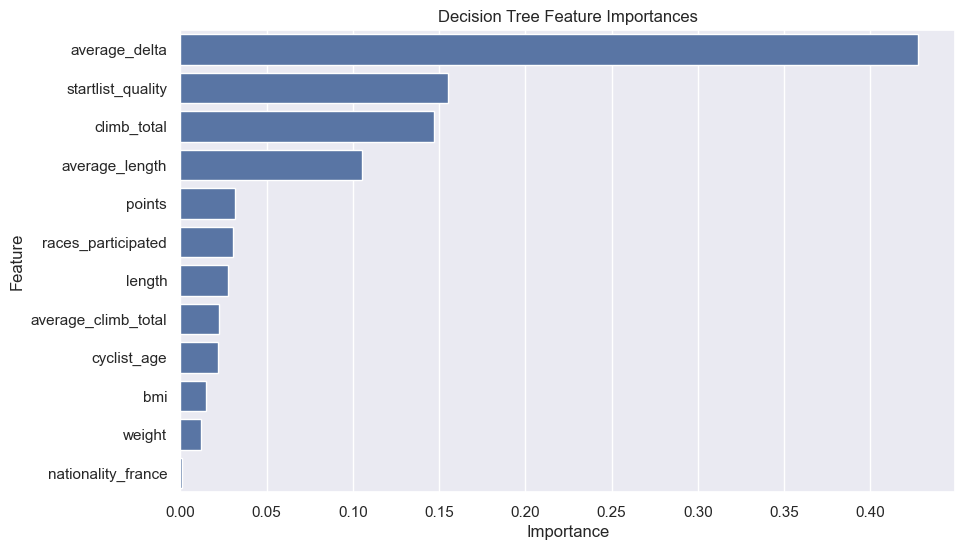
\includegraphics[width=0.9\linewidth]{builtin-dt.png}
\caption{Feature Importance of Decision Tree Model}
\label{fig:decision_tree_importance}
\end{figure}

\subsubsubsection{Using SHAP Values}
Even though the built-in feature importance metric already provides clear information about the importance of each feature, we wanted to also test the SHAP method to see if it would provide the same results.

As expected, the results are really similar \ref{fig:shapdt}.

\begin{figure}[H]
    \centering
    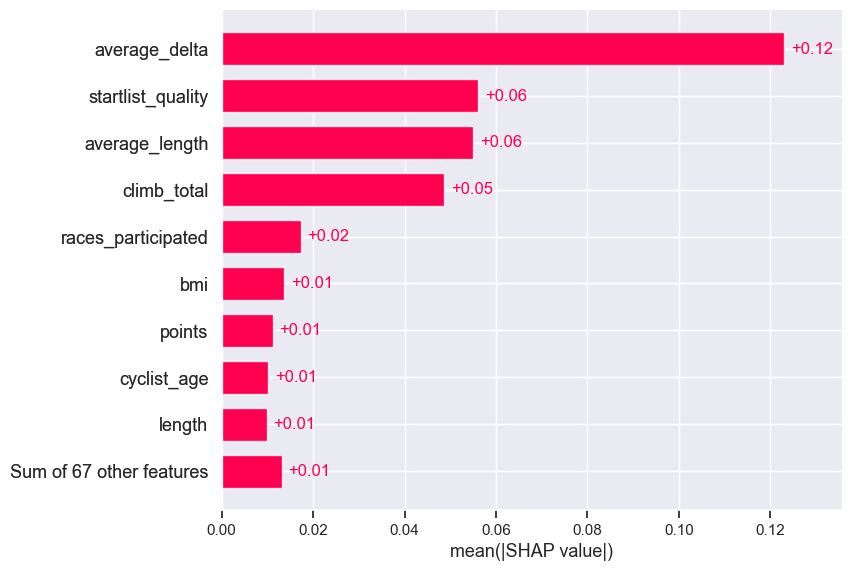
\includegraphics[width=0.75\linewidth]{shapdt.png}
    \caption{SHAP Feature Importance of Decision Tree Model}
    \label{fig:shapdt}
\end{figure}

SHAP also enables us to visualize waterfall plots for individual predictions, which show how each feature contributes to the final prediction. Figure \ref{fig:shapwaterfalldt} shows the waterfall plot for a single prediction. The plot shows that the prediction was made by adding the contributions of each feature, with the most influential features at the top of the plot.



\begin{figure}[H]
    \centering
    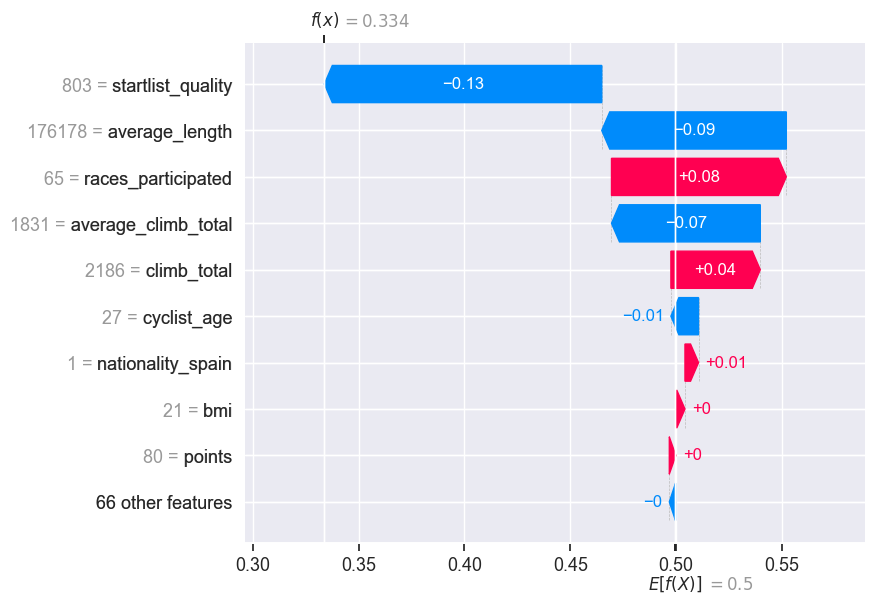
\includegraphics[width=0.5\linewidth]{image.png}
    \caption{Waterfall plot on a particular instance}
    \label{fig:shapwaterfalldt}
\end{figure}


To evaluate the fidelity of SHAP, we also compared it to the built-in importance metric, getting really similar results \ref{fig:compshap}

\begin{figure}[H]
    \centering
    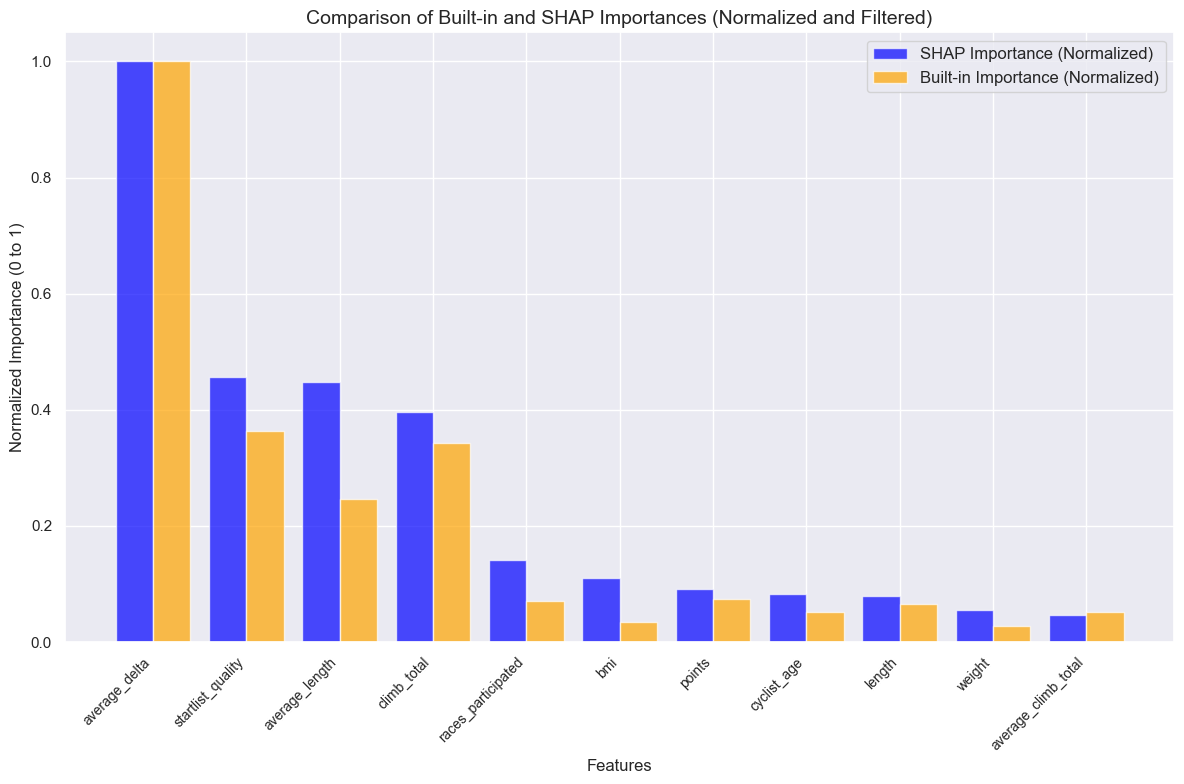
\includegraphics[width=0.75\linewidth]{compshap.png}
    \caption{Comparison of SHAP and built-in importance metric for tree models}
    \label{fig:compshap}
\end{figure}


\subsubsection{Explaining Model Behavior}

\subsubsection{Rule Explanation}
Decision Trees are a transparent model, so we analyzed the tree structure and the decision rules at each node. We can observe it by looking at the tree visualization \ref{fig:dt}.

\begin{figure}[H]
    \centering
    
\includegraphics[width=1\linewidth]{dt.png}
    \caption{Enter Caption}
    \label{fig:dt}
\end{figure}

The tree is composed by 127 nodes, resulting in a big number of rules to be examined to comprehend the model as a whole. By examining individual instances instead, we can focus on the rules involved in the decision-making of the specific instance. 

We were able to identify how specific thresholds in key features, such as \texttt{climb\_total}, influenced the final prediction, confirming the importance of these features. 

For example, let's take a particular instance (instance 0, which was classified as is\_top\_20=1). The rules involved in its classifications (i.e.: the path followed from the root to the leaf) are:

\begin{itemize}
    \item \texttt{average\_delta} \textgreater 334.5
    \item \texttt{climb\_total} \textless= 2660.0
    \item \texttt{average\_length} \textgreater 166136.5
    \item \texttt{startlist\_quality} \textless= 848.5
    \item \texttt{average\_delta} \textgreater 464.5
    \item \texttt{startlist\_quality} \textgreater 428.5
    \item \texttt{races\_participated} \textgreater 128.5
\end{itemize}
Leaf node 174 was reached, with a prediction of \texttt{[[0.44924285, 0.55075715]]}.

\subsubsection{Counterfactual Instances}

We used DiCE to generate counterfactuals, which help us understand how small changes in input features could alter predictions. By making minimal adjustments to the values of key features, we observed how the predicted class would change. This process revealed that certain features had a more substantial impact on predictions, providing valuable insights into the model's sensitivity to specific inputs.

\paragraph{Original Instance (Outcome: 0)} Here is the original instance that resulted in a prediction of 0 (not in the top 20):

\[
\begin{array}{|c|c|c|c|c|c|c|c|c|c|c|}
\hline
\text{points} & \text{length} & \text{climb\_total} & \text{startlist\_quality} & \text{cyclist\_age} & \text{weight} & \text{bmi} & \text{races\_participated} & \text{average\_climb\_total} & \text{average\_length} \\
\hline
225.0 & 196200.0 & 1652.0 & 727.0 & 24.0 & 71.0 & 20.3 & 53.0 & 2143.0 & 192015.0 \\
\hline
\end{array}
\]

\paragraph{Diverse Counterfactual Set (New Outcome: 1)} By generating counterfactuals, we adjusted key features to explore how minimal changes in inputs could shift the outcome. The table below shows three counterfactual instances that resulted in a prediction of 1 (top 20). These changes highlight which features have a significant impact on improving the prediction. For instance, small increases in \texttt{bmi} and \texttt{races\_participated} were sufficient to change the predicted outcome from 0 to 1 in certain cases.

\[
\begin{array}{|c|c|c|c|c|c|c|c|c|c|c|}
\hline
\text{points} & \text{length} & \text{climb\_total} & \text{startlist\_quality} & \text{cyclist\_age} & \text{weight} & \text{bmi} & \text{races\_participated} & \text{average\_climb\_total} & \text{average\_length} & \text{is\_top\_20} \\
\hline
- & - & - & - & - & - & 24.6 & - & - & - & 1.0 \\
- & - & - & - & - & - & 21.0 & 315.3 & - & - & 1.0 \\
- & - & - & - & - & - & 24.7 & - & - & - & 1.0 \\
\hline
\end{array}
\]

We observe, in particular, that a change in the bmi attribute would change the prediction, according to these counterfactuals.
In fact, in each of these counterfactuals, the \texttt{bmi} value was adjusted slightly.










\subsection{Explanation for the Neural Network Model}

\subsubsection{Feature Importance}

Understanding the importance of features in the neural network model can be more challenging due to its complexity, but several techniques can be used to understand which features have the most significant impact on predictions.

\paragraph{Examples on Instances: SHAP Waterfall Plot Analysis}

One effective method for explaining the model's decisions is by using SHAP (SHapley Additive exPlanations) values. SHAP provides a unified approach to explain the contributions of each feature to the model's output for individual instances.

For instance, a SHAP waterfall plot shows how the prediction is broken down by individual feature contributions. This method allows us to interpret the influence of each feature on the model’s decision. In Figure \ref{fig:shap_nn}, we show the waterfall plot for a specific instance. The plot reveals that features such as \texttt{climb\_total}, \texttt{startlist\_quality}, and \texttt{races\_participated} are the most influential in driving the final prediction.

\begin{figure}[H]
    \centering
    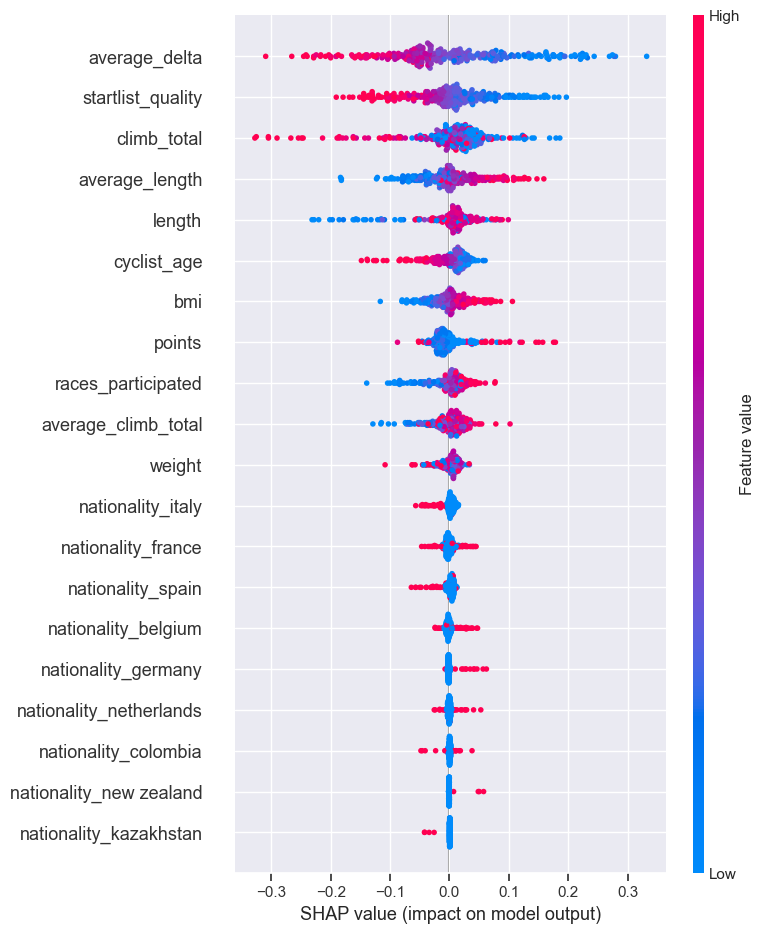
\includegraphics[width=0.75\linewidth]{shap_nn.png}
    \caption{SHAP Waterfall Plot for Neural Network Model}
    \label{fig:shap_nn}
\end{figure}

This method gives a clear picture of how each feature contributes to a prediction, allowing us to make transparent conclusions about the model’s behavior for specific instances.


A summary plot of SHAP values for all instances can also provide a global view of feature importance. This analysis can help identify which features are consistently influential across the dataset and provide insights into the model's overall behavior.

\begin{figure}[H]
    \centering
    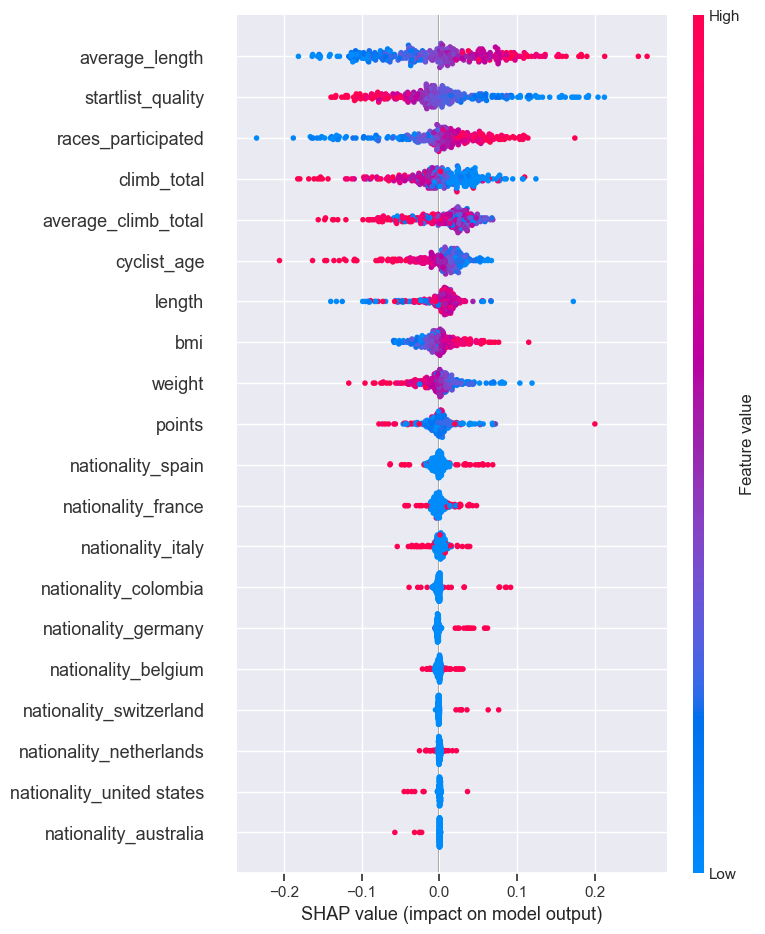
\includegraphics[width=0.75\linewidth]{shap_summary_nn.png}
    \caption{SHAP Summary Plot for Neural Network Model}
    \label{fig:shap_summary_nn}
\end{figure}

In addition to SHAP, we also used LIME (Local Interpretable Model-Agnostic Explanations) as a surrogate model to explain the neural network’s decisions. LIME generates a local interpretable model for a given prediction by approximating the complex neural network with a simpler, interpretable model (such as a linear model) in the vicinity of the prediction.

The LIME scores obtained are comparable to SHAP values and provide a similar interpretation of feature importance.


\subsubsection{Rule Explanation}

Neural networks, unlike decision trees, are not inherently interpretable, as they rely on complex layers of interconnected nodes. Howe

While the model itself doesn't have explicit rules like a decision tree, the analyses we performed and the counterfactual instances suggest that specific thresholds and combinations of features, such as a high \texttt{races\_participated} value, an optimal \texttt{bmi} or a small \texttt{average\_delta}, can significantly shift the predicted outcome.

We attempted to use the \texttt{LIMxailib.explainers.lore\_explainer} to extract rules from the neural network model. However, the computation time for a single instance was excessively long, even though we tried different configurations, so we were unable to extract rules using this method.




\subsubsection{Counterfactual Instances}

We also explored counterfactual explanations for the neural network model using DiCE to understand how slight changes in feature values could alter predictions. Just as with the Decision Tree model, counterfactuals provide a valuable tool for interpreting the decision boundaries of the neural network.

\paragraph{Observing the Counterfactuals}

One of the counterfactuals generated for the neural network model showed that small adjustments in features like \texttt{bmi} and \texttt{average\_delta} can change the predicted outcome significantly. For instance, increasing the \texttt{bmi} value to around 24.5 and \texttt{races\_participated} to over 150 resulted in a change from a prediction of 0 (not in top 20) to 1 (top 20).

We observed that while the neural network model is more complex than decision trees, its sensitivity to key features like \texttt{races\_participated} and \texttt{average\_delta} aligns with the trends seen in the decision tree. This provides useful insights into the features that influence the predictions of cycling performance in both models.



















\subsection{Final Observations}
The patterns identified in the model outputs largely align with what we learned through data exploration and clustering analysis, particularly the importance of \texttt{average\_delta}, which also aligns with intuition about the impact of previous performance on future results. 

However, some models, particularly the neural network, uncovered new patterns that were less evident in earlier analyses. For example, excessive race participation was found to negatively impact performance.

While most predictions align with expectations, some anomalies deserve further investigation. For example, there are many cases where a high-quality start list was associated with a lower likelihood of top finishes. This might suggest that the model may disproportionately focus on race-specific characteristics rather than cyclist-specific attributes. This limitation may come from a lack of cyclist-focused features in the dataset.

Overall, the models performed reasonably well, given the complexity of the prediction task, but there is room for improvement. These observations highlight the potential benefit of integrating new features, either from external data sources or through the creation of novel attributes. Enhancing the dataset with cyclist-specific charateristics could shift the model’s focus from race attributes to the individual cyclist, potentially leading to more accurate predctions.



\end{document}